\documentclass[11pt]{article} 
%\documentclass[9pt,twocolumn,twoside]{pnas-new}
%\documentclass[numsec,webpdf,modern,medium,namedate]{oup-authoring-template}
% Use the lineno option to display guide line numbers if required.
%\onecolumn

%\usepackage[foot]{amsaddr}

\newcommand\suppSecProofFunctionalForms{S1}
\newcommand\suppSecProofOptimizationConvergence{S2}
\newcommand\suppSecFeynmanKac{S3}
\newcommand\suppSecProofTriangularArrays{S4}
\newcommand\suppSecProofConsistency{S5}
\newcommand\suppSecProofBiasVar{S6}
\newcommand\suppSecBayesFigs{S7}
\newcommand\suppSecBaselineJustification{S8}
\newcommand\suppSecAlgorithmicParameters{S9}

\usepackage{natbib}
\usepackage{hyperref}
%\hypersetup{colorlinks=true, citecolor=blue, linkcolor=blue, urlcolor=blue}
\hypersetup{hidelinks}


\usepackage{booktabs}
% \newcommand{\description}{}
\usepackage{enumitem}

\newcommand\new[1]{\textcolor{red}{#1}}
\newcommand\eic[1]{\textcolor{orange}{#1}}
\newcommand\aja[1]{\textcolor{blue}{#1}}

\newcommand\arxiv[2]{#1} % 1st argument for arxiv format
% also, swich to \documentclass[11pt]{article} for arxiv format

\input{macros}

\usepackage{tabto}


%\arxiv{
  \usepackage{fullpage}
  \usepackage{algorithm}
  \usepackage[noend]{algpseudocode}
  \usepackage{xcolor}
%  \usepackage{tikz}
%  \bibliographystyle{ieeetr}
%}{
  
%% \theoremstyle{thmstyleone}%
%% \newtheorem{theorem}{Theorem}%  meant for continuous numbers
%% %%\newtheorem{theorem}{Theorem}[section]% meant for sectionwise numbers
%% %% optional argument [theorem] produces theorem numbering sequence instead of independent numbers for Proposition
%% \newtheorem{proposition}[theorem]{Proposition}%
%% %%\newtheorem{proposition}{Proposition}% to get separate numbers for theorem and proposition etc.
%% \theoremstyle{thmstyletwo}%w
%% \newtheorem{example}{Example}%
%% \newtheorem{remark}{Remark}%
%% \theoremstyle{thmstylethree}%
%% \newtheorem{definition}{Definition}
%% \usepackage[doublespacing]{setspace}
%% \usepackage[fontsize=12pt]{fontsize}}



\AtEndDocument{\refstepcounter{thm}\label{finalthm}}
\AtEndDocument{\refstepcounter{lem}\label{finallem}}
\AtEndDocument{\refstepcounter{defn}\label{finaldefn}}
\AtEndDocument{\refstepcounter{prop}\label{finalprop}}
\AtEndDocument{\refstepcounter{aspt}\label{finalaspt}}
\AtEndDocument{\refstepcounter{figure}\label{finalfig}}


\begin{document}

\title{\articleTitle}

\author{K. Tan$^{1}$, A. J. Abkemeier$^{2}$, G. Hooker$^{1}$ and E. L. Ionides$^{2}$
  \vspace{3ex}\\
  \small{$^{1}$Department of Statistics, University of Pennsylvania}\\
  \small{$^{2}$Department of Statistics, University of Michigan}}

\date{}

\maketitle

\begin{abstract}
  Automatic differentiation (AD) has driven recent advances in machine learning, including deep neural networks and Hamiltonian Markov Chain Monte Carlo methods. Partially observed nonlinear stochastic dynamical systems have proved resistant to AD techniques because widely used particle filter algorithms yield an estimated likelihood function that is discontinuous as a function of the model parameters. To resolve this, we create a theoretical framework that embeds two existing AD particle filter methods within a new class of algorithms. This new class permits a bias-variance tradeoff and hence a mean squared error substantially lower than the existing algorithms. This allows us to develop likelihood maximization algorithms suited to the Monte Carlo properties of the AD gradient estimate. Our algorithms require only a differentiable simulator for the latent dynamic system; by contrast, most previous approaches to AD likelihood maximization for particle filters require access to the system's transition probabilities. Numerical results indicate that a hybrid algorithm, using AD to refine a coarse solution from an iterated filtering algorithm, shows substantial improvement on current state-of-the-art methods on a challenging scientific benchmark problem.
\end{abstract}

% \keywords{Sequential Monte Carlo, Automatic Differentiation, Particle Filter, Markov Process, Likelihood}


\section{Introduction}

Many scientific models involve highly nonlinear stochastic dynamic systems possessing significant random variation in both the process dynamics and the measurements.
Commonly, the latent system is modeled as a Markov process, giving rise to a partially observed Markov process (POMP) model, also known as a hidden Markov models or a state space model.
POMP models arise in fields as diverse as optimal control \citep{singh22}, epidemiology \citep{he10, stocks17}, ecology \citep{knape12} and finance \citep{kim08, breto14}.
Despite their ubiquity, estimation and inference for this broad class of models remains a challenging problem.
We develop full-information plug-and-play inference for POMP models that takes advantage of automatic differentiation (AD) computation while controlling the Monte Carlo bias and variance of the resulting estimator.
These desiderata have not previously been combined, and we discuss each component in turn.

Full-information methods are those which make statistically efficient use of data, typically via likelihood-based or Bayesian methods that avoid dependence on summary statistics.
The particle filter, also known as sequential Monte Carlo, serves as the foundation for various full-information inference algorithms for POMP models, since it provides an unbiased estimate of the likelihood function \citep{delMoral04}, enabling Bayesian inference via particle Markov chain Monte Carlo \citep{andrieu10} and likelihood-based inference via iterated filtering algorithms IF1 \citep{ionides06-pnas} and IF2 \citep{ionides15}.

An inference algorithm for a POMP model is said to be plug-and-play if it does not need to evaluate the transition density of the latent Markov process, enabling an arbitrary model simulator to be plugged into the algorithm, a convenient property that facilitates scientific discovery \citep{he10}.
Some plug-and-play methods depend on the construction of low-dimensional summary statistics \citep{wood10,toni09}, sacrificing statistical efficiency for computational convenience.
Here, our mission is to extend current computational capability among methods that maintain statistical efficiency and the plug-and-play property.
Plug-and-play methods are sometimes called likelihood-free \citep{owen15}, and it may be counter-intuitive that likelihood-based inference is possible using likelihood-free methods. 
Basic particle filters, also known as boostrap filters, possess the plug-and-play property.
Iterated particle filtering algorithms, such as IF1 and IF2, have shown that plug-and-play likelihood maximization is practical in various scientific investigations \citep{king08,blake14,pons-salort18,subramanian21,fox22,drake23}.
However, iterated filtering algorithms have slow convergence near the MLE \citep{doucet13}

Advances in AD for gradient estimation using particle filters \citep{naesseth18, jonschkowski18, corenflos21, scibior21, singh22} have drawn attention to AD as a tool for inference in POMP models.
Widespread adoption of these approaches have been limited by their bias \citep{naesseth18, jonschkowski18}, high variance \citep{poyiadjis11, scibior21}, computational expense quadratic in the number of particles \citep{corenflos21, chen24}, or by the loss of the plug-and-play property \citep{poyiadjis11, scibior21, singh22, chen24}.
We present a new algorithm which (for reasons which will be discussed later) we call a {\it Differentiated Measurement Off-Parameter} (DMOP) particle filter.
DMOP corresponds to the derivative of a smooth variant of the particle filter that we call MOP, though DMOP is conveniently calculated using AD without the need to actually implement the full MOP filter.
MOP has the special property that, unlike most particle filters, the gradient of the filtered log-likelihood estimate provides a consistent estimate of the gradient of the log-likelihood.
Particle filters have previously been adapted to provide a smooth estimate of the likelihood function \citep{svensson18,malik11}, but MOP and DMOP differ from these by possessing the plug-and-play property.

DMOP trades bias against variance via a discount factor, $\alpha \in [0,1]$.
We find that DMOP-$\alpha$ posesses a bias-variance tradeoff that permits both low bias and low variance for suitable choices of $\alpha$ strictly in $(0,1)$, both in theory (Theorem \ref{thm:mop-biasvar}) and practice (Figure \ref{fig:biasvar}).
Theorem~\ref{thm:mop-functional-forms} shows that DMOP-$\alpha$ coincides with the biased gradient estimator of \cite{naesseth18} when $\alpha=0$.
In a limit as the number of particles increases, Theorem~\ref{thm:mop-functional-forms} also shows that DMOP-$\alpha$ with $\alpha=1$ matches the high-variance gradient estimate from \cite{poyiadjis11} and \cite{scibior21}.
In this case, the variance can become prohibitively high, as discovered by these researchers and others \citep{arya22}.
However, the variance rapidly reduces as $\alpha$ decreases, and so a choice of $\alpha$ close to one can provide a low-bias, low-variance, plug-and-play gradient estimate with computational scaling linear in the number of particles.

In practice, likelihood optimization via gradient descent with DMOP-$\alpha$ converges quickly within a neighborhood of the maximum but struggles to reach this neighborhood in the presence of local minima and saddle points.
By contrast, iterated filtering algorithms provide a relatively fast and stable way to identify this neighborhood.
We therefore build a simple but effective hybrid algorithm called {\it Iterated Filtering with Automatic Differentiation} (IFAD) that warm-starts first-order or second-order gradient methods with a preliminary solution obtained from iterated filtering.
We implement our algorithm using JAX \citep{jax}, which also enables us to take advantage of graphical processing unit (GPU) hardware.
Our methodology is provided in an open-source software library, Pypomp \citep{abkemeier25}.

Promising numerical results indicate that IFAD beats IF2 (and by the numerical results of \cite{ionides15}, also IF1 and the Liu-West filter \citep{liuwest01}) on a challenging problem in epidemiology, the Dhaka cholera model of \cite{king08}.
Empirically, the benchmark tests suggest that IFAD is the most significant methodological advance since \cite{ionides15} for plug-and-play statistical inference on POMP models.
The choice of models and methods for benchmarking is justified in Section~\suppSecBaselineJustification. 

We also demonstrate empirical advances using DMOP-$\alpha$ for Bayesian inference.
In Section~\ref{sec:bayes}, we use the DMOP-$\alpha$ gradient estimates within a No-U-Turn Sampler (NUTS) \citep{homan14} in conjunction with an empirical Bayes-type prior estimated with IF2 to reduce the burn-in period of particle MCMC \citep{andrieu10} on the Dhaka cholera model of \cite{king08} from the $700,000$ iterations in \cite{fasiolo16} to just $500$.
To the best of our knowledge, attaining rapid mixing on this challenging problem has not previously been achieved. 

\section{Problem Setup}

Consider an unobserved Markov process $\{X(t),t  \geq t_0\}$, with discrete-time observations $Y_1,...,Y_N$ realized at values $y_1^*,\dots,y_N^*$ with times $t_1,\dots, t_N$.
The process is parameterized by an unknown parameter $\theta \in \Theta \subseteq \R^p$, where the state $X(t)$ takes values in the state space $\gX \subseteq \R^d$, the observations $Y_n$ take values in $\gY,$ and we write $X_n = X(t_n)$. We suppose that the discrete-time latent process model has a density $f_{X_n|X_{n-1}}\left(x_{n} \mid x_{n-1}; \theta\right)$.
The existence of this density is necessary to define the likelihood function, but plug-and-play algorithms do not explicitly evaluate it.
Instead, they have access to a corresponding simulator, which write as $\process_n\left(x_n\mid x_{n-1}; \theta\right)$.
We set $f_{Y_n|X_n}\left(y_n \mid x_n; \theta\right)$ to be the measurement density, which  can be directly evaluated. 
We call $f_{X_{1:n}|Y_{1:n}}(x_{1:n}|y_{1:n}^*; \theta)$ the posterior distribution of states, and $f_{X_{n}|Y_{1:n}}(x_n|y_{1:n}^*; \theta)$ the filtering distribution at time $t_n$.
All joint and conditional densities are defined on a probability space $(\Omega, \Sigma, \prob)$ which is also assumed to enable construction of independent replicates and all random variables defined in our algorithms.
For the algorithmic interpretation of our theory, we identify the random number seed with an element of the sample space $\omega \in \Omega$.
The random seed determines the sequence of pseudo-random numbers generated by a computer, just as $\omega\in\Omega$ generates the sequence of random variables.

\section{Off-Parameter Particle Filters}

The {\it Measurement Off-Parameter with discount factor} $\alpha$ (MOP-$\alpha$), particle filter is defined by the pseudocode in Algorithm~\ref{alg:mop}.
Note that this algorithm has the plug-and-play property.
We suppose that the simulator is a differentiable function of $\theta$ for every fixed $\omega$.
This condition is equivalent to the {\it reparameterization trick} \citep{corenflos21}; by writing the generated random numbers as parameter-dependent transformation from a reference distribution---e.g., the quantile transform of a uniform random variable---we can differentiate their values, and hence the simulation, with respect to parameters.
The discrete resampling step of the bootstrap particle filter has been the primary point of concern for the use of AD to estimate derivatives for particle filters.
The discontinuity of this resampling (as a function of $\theta$, for fixed $\omega$) means that the derivative of the expectation is not consistently estimated by the expectation of the derivative. 
MOP-$\alpha$ is a mathematical construction designed to avoid this discontinuity.
We begin with a filter that resamples particles with weights calculated at a baseline parameter value, $\phi$, and then corrects these weights to target the filtering distribution at another parameter value, $\theta$, yielding the name {\it measurement off-parameter}.
The terminology is chosen by analogy with similar {\it off-policy} algorithms used for reinforcement learning in which a policy that was not implemented is evaluated by reweighting the rewards of the policy that was actually applied.
If we fix $\omega$ and $\phi$, the sample indices do not change with $\theta$, but the re-weighting scheme does, allowing MOP-$\alpha$ to be differentiated with respect to $\theta$.
When $\theta = \phi$, we have $w_{n,j}^{P,\theta} = w_{n-1,j}^{F,\theta} = 1$ and MOP-$\alpha$ reduces  to the standard particle filter; this is the setting we use in practice,  but use the construction allows us to define a derivative.
One can think of MOP-$\alpha$ as reconstructing local smooth approximations of the discontinuous likelihood estimates produced by a particle filter for a fixed number of particles $J$ and fixed seed $\omega$.
These approximate the likelihood at $\theta$ in a neighborhood around $\phi$, with the intent that differentiating these smooth log-likelihood reconstructions yields a score estimate.

DMOP-$\alpha$ (Algorithm~\ref{alg:dmop}) computes the fixed-seed derivative of the likelihood estimate obtained by MOP-$\alpha$ at $\theta=\phi$.
To better understand the implementation in DMOP-$\alpha$, we review some background for AD.
 Standard AD consists of two evaluation passes: a forward pass in which the function is evaluated and a graph built of the evaluation process, followed by a backward pass where the derivative is evaluated by recursive use of the chain rule on the computation graph \citep{griewank08}.  
  The two evaluation passes in MOP-$\alpha$ at $\phi$ and $\theta$ correspond to the two AD evaluation passes in DMOP-$\alpha$.
  Differentiation of MOP-$\alpha$ with respect to $\theta$ requires a preliminary evaluation at $\phi$ and subsequent differentiation with respect to $\theta$ for the second pass which we obtain through AD.
In practice, however, we only work in the $\theta = \phi$ setting in which case MOP-$\alpha$ corresponds to the standard particle filter and we only need to make one pass.
In order to apply AD in this setting without using two passes, we must both instantiate the weighting scheme (even though the weights are always 1) and distinguish which components of the weights correspond to which pass.
This can be achieved using the {\it stop-gradient} capability that appears in Algorithm~\ref{alg:dmop} where its application in the weight correction step indicates that AD should apply the chain rule to the numerator but not the denominator of the correction; note that this construction yields weights which are always 1, but which also have non-zero derivatives.  
  
  
\begin{figure}[htbp!]
  \centering
    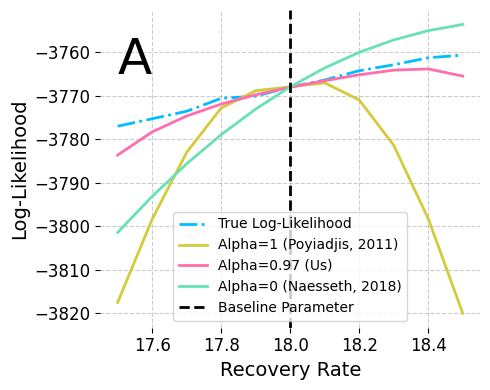
\includegraphics[width=\textwidth/\real{2.2}]{imgs/095/mop.png}
    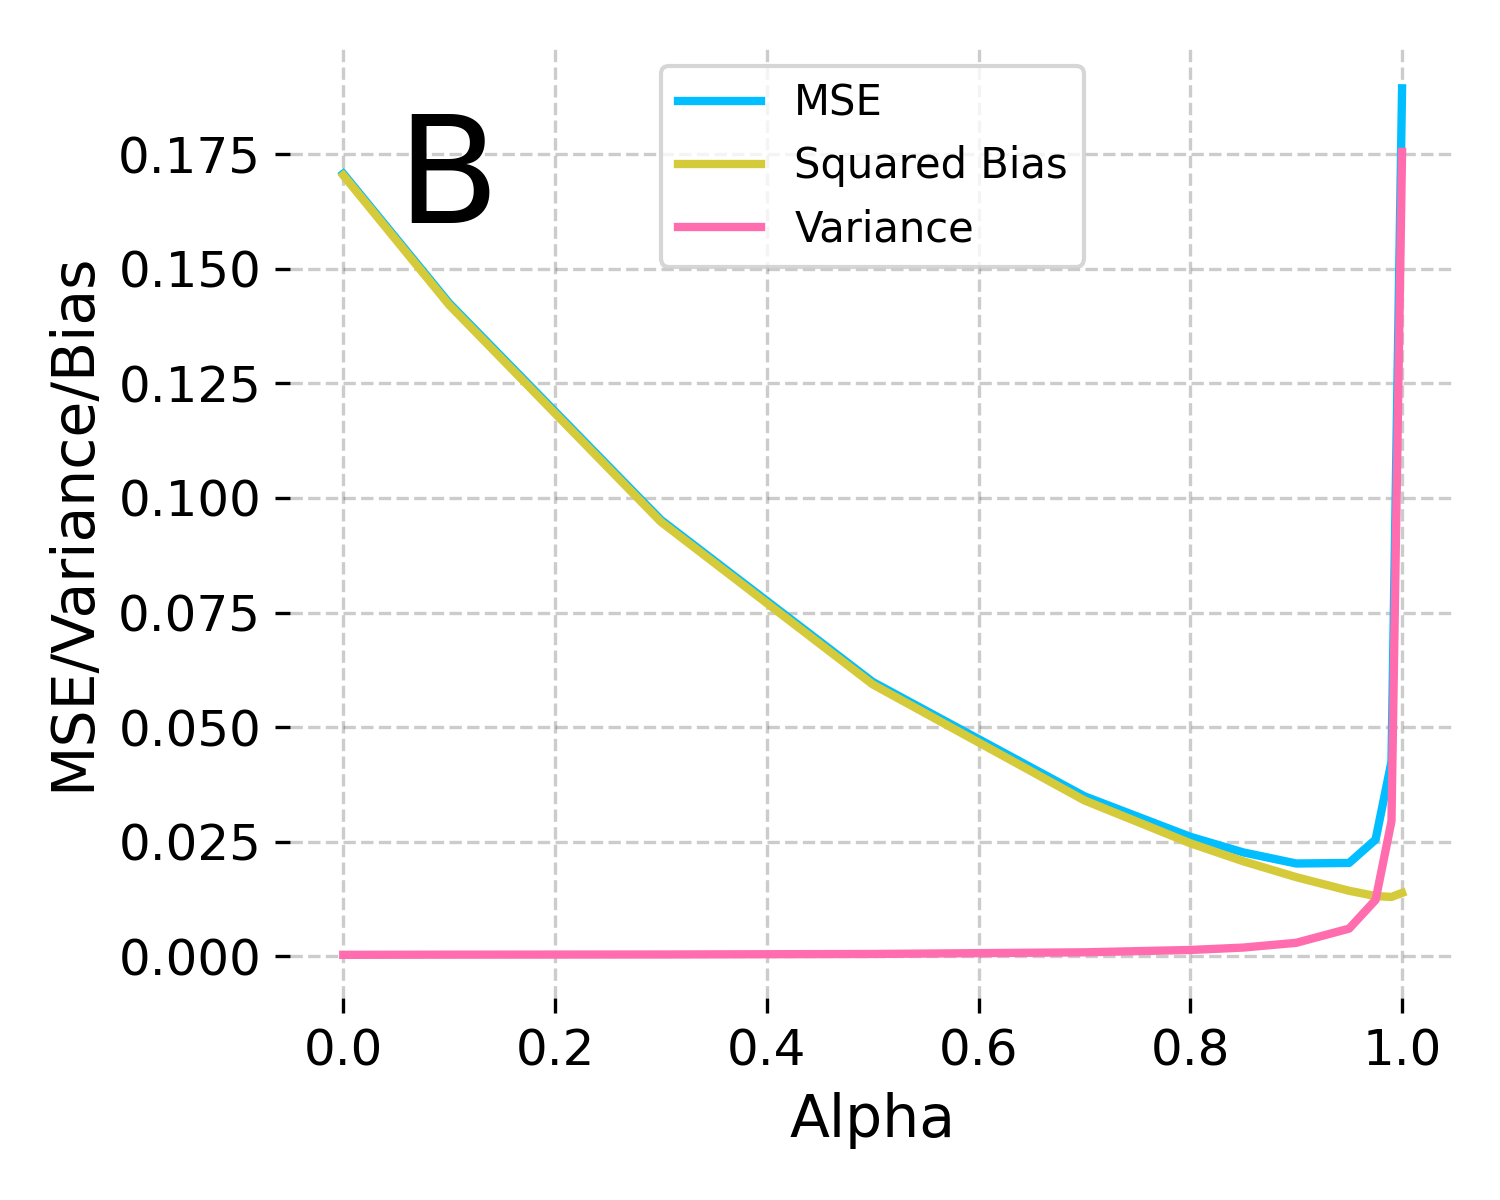
\includegraphics[width=\textwidth/\real{2.2}]{imgs/095/biasvar.png}
    \caption{\textbf{A:} Non‐differentiable likelihood estimates and smooth off‐parameter approximations that hold locally around the baseline parameter $\phi$. \textbf{B:} Illustration of the bias-variance tradeoff induced by the discounting hyperparameter $\alpha$. We display the MSE of score estimates for the recovery rate at the MLE for the Dhaka cholera model of \cite{king08}. Our novel contribution of $\alpha \in (0,1)$ significantly improves the quality of the likelihood approximation and the score estimates.}
    \label{fig:biasvar}
\end{figure}


\begin{algorithm}[htbp!]
	\caption{MOP-$\alpha$}
    \label{alg:mop}
	     \textbf{Input:} Number of particles $J$, timesteps $N$, measurement model $f_{Y_n|X_n}(y_n^*|x_n, \theta)$, simulator $\process_n(\cdot|x_n; \theta)$, evaluation parameter $\theta$, baseline parameter $\phi$, seed $\omega$.
      
        \textbf{First pass:} Set $\theta=\phi$ and fix $\omega$, yielding $X_{n,j}^{P,\phi}$, $X_{n,j}^{F,\phi}$, $g^{\phi}_{n,j}$.
            
        \textbf{Second pass:}
        Fix $\omega$, and filter at $\theta\neq \phi$:
            
		\textbf{Initialize } particles ${X}_{0,j}^{F,\theta}\sim {f}_{{X}_{0}}\left(\cdot\giventh{\theta}\right)$, weights $w^{F,\theta}_{0,j}= 1$. \newline
		\textbf{For} $n=1,...,N$: \newline
            \hspace*{4mm} Accumulate discounted weights, $w_{n,j}^{P,\theta} = \big(w_{n-1,j}^{F,\theta}\big)^\alpha$.\newline
            \hspace*{4mm} Simulate process model,
            ${X}_{n,j}^{P,\theta}\sim \process_n\big(\cdot|{X}_{n-1,j}^{F, \theta};{\theta}\big)$. \newline
            \hspace*{4mm} Measurement density,
            $g^{\theta}_{n,j}={f}_{{Y}_{n}|{X}_{n}}(y_{n}^{*}|{X}_{n,j}^{P,\theta}\giventh{\theta})$. \newline
            \hspace*{4mm} Compute $L_n^{B,\theta,\alpha} ={\sum_{j=1}^Jg^\theta_{n,j} \, w^{P,\theta}_{n,j}}\, \big/\, {\sum_{j=1}^J  w^{P,\theta}_{n,j}}$. \newline
            \hspace*{4mm} Conditional likelihood under $\phi$,
            $L_n^{\phi} = \frac{1}{J}\sum_{m=1}^{J}g^{\phi}_{n,m}$.\newline
            \hspace*{4mm} Select resampling indices $k_{1:J}$ with $\prob\big(k_{j}=m\big) \propto g^{\phi}_{n,m}$. \newline
            \hspace*{4mm} Obtain resampled particles ${X}_{n,j}^{F,\theta}={X}_{n,k_{j}}^{P,\theta}$. \newline
            \hspace*{4mm} Calculate corrected weights
            $w_{n,j}^{F,\theta}= w^{P,\theta}_{n,k_j} \, g^{\theta}_{n,k_j} \, \big/ \, { g^{\phi}_{n,k_j}}$.\newline
            \hspace*{4mm} Compute $ L_n^{A,\theta,\alpha} = L_n^\phi\cdot {\sum_{j=1}^J w^{F,\theta}_{n,j}} \, \big/ \, {\sum_{j=1}^J  w^{P,\theta}_{n,j}}$.\newline
	    \textbf{Return:} likelihood estimate $\hat{\lik}^A(\theta) = \prod_{n=1}^N L_n^{A,\theta,\alpha}$ or $\hat{\lik}^B(\theta) = \prod_{n=1}^N L_n^{B,\theta,\alpha}$,
            log-likelihood $\hat{\loglik}^A(\theta)=\log\big(\hat{\lik}^A(\theta)\big)$ or  $\hat{\loglik}^B(\theta)=\log\big(\hat{\lik}^B(\theta)\big)$,
            and filtering distributions $\{(X_{n,j}^{F, \theta}, w^{F,\theta}_{n,j})\}_{n,j=1}^{N,J}.$
\end{algorithm}


\begin{algorithm}[htbp!]
	\caption{DMOP-$\alpha$}
    \label{alg:dmop}
	     \textbf{Input:} Number of particles $J$, timesteps $N$, measurement model $f_{Y_n|X_n}(y_n^*|x_n, \theta)$, simulator $\process_n(\cdot|x_n; \theta)$, parameter $\theta$.
      
             \textbf{Forward pass:} AD constructs a computation graph for the likelihood estimate, $\hat{\lik}^A(\theta) = \prod_{n=1}^N L_n^{A,\theta,\alpha}$ or $\hat{\lik}^B(\theta) = \prod_{n=1}^N L_n^{B,\theta,\alpha}$. 
            
        \textbf{Backward pass:} AD evaluates the gradient estimate, $\hat{\mathcal{D}}^A(\theta)$ or  $\hat{\mathcal{D}}^B(\theta)$.
            
		\textbf{Initialize } particles ${X}_{0,j}^{F,\theta}\sim {f}_{{X}_{0}}\left(\cdot\giventh{\theta}\right)$, weights $w^{F,\theta}_{0,j}= 1$. \newline
		\textbf{For} $n=1,...,N$: \newline
            \hspace*{4mm} Accumulate discounted weights, $w_{n,j}^{P,\theta} = \big(w_{n-1,j}^{F,\theta}\big)^\alpha$.\newline
            \hspace*{4mm} Simulate process model,
            ${X}_{n,j}^{P,\theta}\sim \process_n\big(\cdot|{X}_{n-1,j}^{F, \theta};{\theta}\big)$. \newline
            \hspace*{4mm} Measurement density,
            $g^{\theta}_{n,j}={f}_{{Y}_{n}|{X}_{n}}(y_{n}^{*}|{X}_{n,j}^{P,\theta}\giventh{\theta})$. \newline
            \hspace*{4mm} Compute $L_n^{B,\theta,\alpha} ={\sum_{j=1}^Jg^\theta_{n,j} \, w^{P,\theta}_{n,j}}\, \big/\, {\sum_{j=1}^J  w^{P,\theta}_{n,j}}$. \newline
%            \hspace*{4mm} Conditional likelihood under $\phi$,
%            $L_n^{\phi} = \frac{1}{J}\sum_{m=1}^{J}g^{\phi}_{n,m}$.\newline
            \hspace*{4mm} Select resampling indices $k_{1:J}$ with $\prob\big(k_{j}=m\big) \propto g^{\theta}_{n,m}$. \newline
            \hspace*{4mm} Obtain resampled particles ${X}_{n,j}^{F,\theta}={X}_{n,k_{j}}^{P,\theta}$. \newline
            \hspace*{4mm} Calculate corrected weights
            $w_{n,j}^{F,\theta}= w^{P,\theta}_{n,k_j} \, g^{\theta}_{n,k_j} \, \big/ \, { \mathtt{stop\_gradient}(g^{\theta}_{n,k_j})}$.\newline
            \hspace*{4mm} Compute $ L_n^{A,\theta,\alpha} = L_n^\phi\cdot {\sum_{j=1}^J w^{F,\theta}_{n,j}} \, \big/ \, {\sum_{j=1}^J  w^{P,\theta}_{n,j}}$.\newline
	    \textbf{Return:} log-likelihood estimate $\hat{\loglik}^A(\theta)= \log\big(\hat{\lik}^A(\theta)\big) = \sum_{n=1}^N \log L_n^{A,\theta,\alpha}$ or $\hat{\loglik}^B(\theta)=\log\big(\hat{\lik}^B(\theta)\big) = \sum_{n=1}^N \log L_n^{B,\theta,\alpha}$, and gradient estimate $\hat{\mathcal{D}}^A(\theta)$ or $\hat{\mathcal{D}}^B(\theta)$.
\end{algorithm}

MOP-$\alpha$ has similarities with \cite{svensson18}, in which particles from a previous run at $\phi$ are reweighted to evaluate the likelihood at any sufficiently nearby parameter $\theta$ for $0$-th order optimization.
However, their method is not plug-and-play because they use transition densities to reweight particles, and the variance of their log-likelihood estimate has an exponential dependence in the horizon, $N$, when $\theta\neq\phi$.
Our approach bypasses these issues -- the first since the reparameterization trick allows us to consider particle paths dependent on $\theta$, and the second as using AD allows us to only evaluate the likelihood and score estimates when $\theta=\phi$. 

\subsection{Some algorithmic details}

The resampling indices, which we write as $k_j \sim \text{Categorical}(g^{\phi}_{n,1},...,g^{\phi}_{n,J})$, are a function of $\phi$ for any value of $\theta$.
For the categorical distribution, we use systematic resampling \citep{arulampalam02,king16} which usually outperforms multinomial resampling.
The finite-sample concentration result used for Theorem~\ref{thm:linear},
however, is stated for multinomial resampling; it does not assert the same
guarantee for the systematic-resampling implementation used in our numerical
work.

In Algorithm~\ref{alg:mop}, the conditional likelihoods are reweighted by a correction factor $w^{P,\theta}_{n,j}$ that accumulates over filtering steps to account for the resampling under $\phi$. 
Writing $g^{\theta}_{n,j}={f}_{{Y}_{n}|{X}_{n}}(y_{n}^{*}|{X}_{n,j}^{P,\theta}\giventh{\theta})$ for the measurement density and $L_n^{\phi} = \frac{1}{J}\sum_{m=1}^{J}g^{\phi}_{n,m}$ for the conditional likelihood estimate under $\phi$, we obtain two estimates of the conditional likelihood under $\theta$,
\begin{equation}
     \label{eq:mop-conditional-likelihood}
     L_n^{B,\theta,\alpha} = \frac{\sum_{j=1}^Jg^\theta_{n,j}\, w^{P,\theta}_{n,j}}{\sum_{j=1}^J  w^{P,\theta}_{n,j}}, \arxiv{\hspace{15mm}}{\;\;}
     L_n^{A,\theta,\alpha} = L_n^\phi\cdot \frac{\sum_{j=1}^J w^{F,\theta}_{n,j}}{\sum_{j=1}^J  w^{P,\theta}_{n,j}},
\end{equation}
where we recursively correct the weights for each particle for the cumulative error incurred by the off-parameter resampling:
\begin{equation}
    \label{eq:weighting-scheme}
    w_{n,j}^{P,\theta} = (w_{n-1,j}^{F,\theta})^\alpha, 
    \arxiv{\hspace{5mm}}{\;}
    w^{F,\theta}_{n,j} = w^{P,\theta}_{n,k_j} \, g^{\theta}_{n,k_j} \, \big/ g^{\phi}_{n,k_j}, 
    \arxiv{\hspace{5mm}}{\;}
    w^{F,\theta}_{0,j}= 1.
\end{equation}
The before-resampling estimate $L_n^{B,\theta,\alpha}$ is preferable in practice, as it has slightly lower variance than the after-resampling estimate $L_n^{A,\theta,\alpha}$, but the latter is useful in deriving properties of the MOP-$\alpha$ gradient estimate such as that in Theorem \ref{thm:mop-functional-forms}.


\subsection{Discounted Weights and a Bias-Variance Tradeoff}

Heuristically, $\alpha$ controls the exponentially decaying memory of MOP and DMOP.
Importantly, $\alpha$ is irrelevant for MOP at $\theta=\phi$ when the weights are always 1 and therefore also irrelevant for the function evaluation in the first pass of DMOP, but crucially not in the second when the gradients are evaluated.
If $\alpha=1$, the gradient of the weights, $w^{P,\theta}_{n,j}$ and $w^{F,\theta}_{n,j}$, accumulates as $n$ increases.
This leads to numerical instability and high variance unless $N$ is small.
For $\alpha<1$, the weights from previous timesteps are discounted as in Equation~(\ref{eq:weighting-scheme}), allowing for lower variance at the expense of bias in the gradient estimate.

When $\alpha=1$, MOP-$1$ maintains complete memory of each particle's ancestral trajectory.
Theorem~\ref{thm:mop-functional-forms} shows that DMOP-$1$ recovers the consistent but high-variance score estimate of \cite{poyiadjis11}. 
When $\alpha=0$, MOP-$0$ considers only single-step transition dynamics, and DMOP-$0$ recovers the low-variance but asymptotically biased score estimate of \cite{naesseth18}.
\cite{scibior21} showed that this matches the gradient of a vanilla particle filter when resampling terms are dropped. 

\begin{thm}[DMOP-$0$ and DMOP-$1$ Functional Forms]
    \label{thm:mop-functional-forms}
    Writing $\nabla_\theta \hat\ell^\alpha(\theta)$ for the gradient estimate yielded by DMOP-$\alpha$ %when $\theta=\phi$ 
    and using the after-resampling conditional likelihood estimate so that $\hat\loglik(\theta)= \log \hat\lik(\theta) = \log \prod_{n=1}^N L_n^{A, \theta, \alpha}$, when $\alpha=0$,
    \begin{equation} \nonumber
        \nabla_\theta \hat\ell^0(\theta) 
        = \frac{1}{J} \sum_{n=1}^N \sum_{j=1}^J \nabla_\theta \log f_{Y_n|X_{n}}(y_n^*|x_{n,j}^{F, \theta}; \theta),
    \end{equation}
    yielding \cite{naesseth18}'s estimator with the bootstrap filter. When $\alpha=1$,
    \begin{equation} \nonumber
        \nabla_\theta \hat{\ell}^1(\theta) 
        = \frac{1}{J}\sum_{j=1}^J \nabla_\theta \log f_{Y_{1:N}|X_{1:N}}\left(y_{1:N}^* | x_{1:n,j}^{A, F,\theta}\right),
    \end{equation}
    yielding the estimator of \cite{poyiadjis11} for the bootstrap filter.
\end{thm}

We defer the proof to the supplement (Section~\suppSecProofFunctionalForms). 
The argument relies on a useful decomposition of the after-resampling estimate $L_n^{A,\theta,\alpha}$, repeated applications of the log-derivative identity that $\nabla_x \log(f(x)) = (\nabla_x f(x))/f(x)$, and noting $\theta=\phi$ implies that $w_{n,j}^{P,\theta}$ evaluates to $1$. 

The result in Theorem \ref{thm:mop-functional-forms} provides mathematical intuition for why \cite{scibior21}'s use of the stop-gradient procedure in the particle filter recovers the estimate of \cite{poyiadjis11}.
When $\theta=\phi$, the correction $g_{n,k_j}^\theta/g_{n,k_j}^\phi$ is equivalent to $g_{n,k_j}^\theta / \text{stop\_gradient}(g_{n,k_j}^\theta)$, and is implemented in this way in practice.
As such, the use of the stop-gradient in \cite{scibior21} can be seen as the MOP-$\alpha$ weight correction for $\alpha=1$, and $\theta=\phi$.


\section{From Gradients to Maximum Likelihood Estimation}

To design an effective procedure for likelihood maximization using DMOP-$\alpha$, we carry out iterated filtering then automatic differentiation (IFAD). 
A basic IFAD approach is presented in Algorithm~\ref{alg:ifad}.
The second stage uses a symmetric positive-definite curvature matrix $B_m$ whose
eigenvalues are kept in a fixed interval $[c,C]$.  A raw particle Hessian or a
quasi-Newton matrix may be spectrally clipped to this interval; the choice
$B_m=I_p$ gives stochastic gradient descent (SGD).
Algorithm~\ref{alg:ifad} is convenient for theoretical analysis, but two further modifications are helpful in practice.
Our best numerical results were obtained by putting the gradient estimate into the Adam optimizer \citep{kingma15} together with learning rate decay. 
Numerical results are provided in Section~\ref{sec:cholera}.

\begin{algorithm}[htbp!]
	\caption{IFAD}
    \label{alg:ifad}
	    \textbf{Input:} Number of particles $J$, timesteps $N$, IF2 cooling schedule $a_m$, AD step size $\eta$, MOP-$\alpha$ discount parameter $\alpha$, spectral bounds $0<c\leq C$, gradient tolerance $\epsilon$, stopping multiplier $\sigma$, maximum AD iterations $M$, and initial value $\theta_0$.\newline
        Run the initial IF2 search under cooling schedule $a_m$ to obtain $\{\Theta_j, j=1,...,J\}$, and set $\theta_0 := J^{-1}\sum_{j=1}^J \Theta_j.$\newline
		\textbf{For} $m=0,\ldots,M-1$: \newline
		\hspace*{4mm} Using fresh random numbers, run Algorithm \ref{alg:mop} to obtain $\hat\loglik(\theta_m)$ and set $g_m := \nabla_{\theta}(-\hat\loglik(\theta_m))$. \newline
		\hspace*{4mm} \textbf{If} $\|g_m\|_2\leq\sigma\epsilon$, \textbf{return} $\hat\theta:=\theta_m$. \newline
		\hspace*{4mm} Choose a symmetric raw curvature estimate $\widetilde B_m$ and clip its eigenvalues to $[c,C]$ to obtain $B_m$. \newline
		\hspace*{4mm} Update $\theta_{m+1} := \theta_m - \eta B_m^{-1} g_m$. \newline
		\textbf{Return} $\hat{\theta} := \theta_M.$
\end{algorithm}

The result below analyzes the specialization of Algorithm~\ref{alg:ifad} that
uses $\alpha=1$, the after-resampling likelihood estimate, and multinomial
resampling.  These restrictions are needed for the stated finite-sample
probability bound.

The convergence of IF2 (and so the first stage of IFAD) to a neighborhood of the MLE happens rapidly in practice. 
%% In the case of the Dhaka cholera model of \cite{king08}, when an aggressive geometric cooling multiplier of 0.95 and initial random walk standard deviation of 0.02 is used, we require no more than 40 iterations of IF2 to obtain an acceptable warm-start. 
However, even when applying much larger amounts of Monte Carlo effort, IF2 fails to get much closer than 3 log-likelihood units of the maximum on this problem (Figure~\ref{fig:boxplot}).
For this example, IF2, without assistance from AD, struggles to reach the inferentially critical region within one log-likelihood unit of the maximum, even when additional computationally intensive techniques are used, such as repeated pruning and profiling,


For a fixed optimization budget, the AD stage has a high-probability linear
convergence rate up to a neighborhood of the MLE that shrinks as the particle
gradient accuracy improves, under the usual smoothness and strong convexity
assumptions, as shown below.

\begin{thm}[Finite-horizon Linear Convergence of IFAD]
\label{thm:linear}\label{thm:mop-convergence}\normalfont
Condition on the IF2 output $\theta_0$, and write $f=-\ell$.  Let
$\mathcal D$ be a deterministic convex region, and let
$\theta^*\in\operatorname{int}(\mathcal D)$ be the unique minimizer of $f$ on
$\mathcal D$ (equivalently, the maximizer of $\ell$).  Assume that
$\mathcal D$ contains every second-stage iterate and every trial point produced
before stopping, and suppose that, for all $\theta\in\mathcal D$,
\[
\gamma I_p\preceq\nabla^2f(\theta)\preceq\Gamma I_p,
\qquad 0<\gamma\leq\Gamma.
\]
Assume (A3) and (A5) uniformly on $\mathcal D$, and define the explicit
constants
\[
R_G=\frac{\bar G}{\underbar G},\qquad
K_N^{\rm pf}=32\sum_{r=0}^N R_G^{3r},\qquad
G'_{\mathcal D}=\sup_{\theta\in\mathcal D}G'(\theta)<\infty.
\]
Fix $M\geq1$, $\delta\in(0,1)$, and $\epsilon>0$.  Let $\mathcal F_m$ contain
the history before the $m$th particle-filter call.  Conditionally on
$\mathcal F_m$, draw the particle-randomness block independently from the
parameter-independent base law, and use multinomial resampling to compute the
after-resampling DMOP-$1$ gradient
$g_m=-\nabla_\theta\hat\ell_J^{A,1}(\theta_m)$.  Choose the integer particle
count to satisfy
\[
J\geq\left\lceil
K_N^{\rm pf}\log\!\left(\frac{6pM}{\delta}\right)
\max\left\{4,
\frac{4pN^2(G'_{\mathcal D})^2}{\epsilon^2}
\right\}\right\rceil.
\]
Let $B_m$ be obtained by clipping the eigenvalues of any symmetric raw
curvature estimate to $[c,C]$, where $0<c\leq C$, and update
$\theta_{m+1}=\theta_m-\eta B_m^{-1}g_m$.  For $\beta\in(0,1)$, choose
\[
0<\eta\leq\frac{c(1-\beta)}{\Gamma},
\qquad
\sigma\geq\frac{2C}{c(1-\beta)}.
\]
Define the stopping time, with the convention that $\min\varnothing=M$, by
\[
\tau=\min\big\{m\in\{0,\ldots,M-1\}:\|g_m\|_2\leq\sigma\epsilon\big\},
\]
and define the simultaneous gradient event
\[
\mathcal E_M=
\bigcap_{m=0}^{\min\{\tau,M-1\}}
\big\{\|g_m-\nabla f(\theta_m)\|_2\leq\epsilon\big\}.
\]
Then $\Pr(\mathcal E_M\mid\theta_0)\geq1-\delta$.  On $\mathcal E_M$, set
\[
q=1-\frac{2\eta\beta\gamma}{C}
\left(\frac{\sigma}{\sigma+1}\right)^2,
\qquad \frac12<q<1,
\]
and $\Delta_m=\ell(\theta^*)-\ell(\theta_m)$.  The following conclusions hold:
\begin{enumerate}[label=(\roman*),leftmargin=7mm,itemsep=1mm]
\item For every $m<\tau$,
$\Delta_{m+1}\leq q\Delta_m$; hence
$\Delta_m\leq q^m\Delta_0$ for $0\leq m\leq\tau$.
\item If $\tau<M$, Algorithm~\ref{alg:ifad} returns $\theta_\tau$ and
\[
\|\nabla f(\theta_\tau)\|_2\leq(\sigma+1)\epsilon,
\qquad
\Delta_\tau\leq\frac{(\sigma+1)^2\epsilon^2}{2\gamma}.
\]
\item If $\tau=M$, Algorithm~\ref{alg:ifad} returns $\theta_M$ and
$\Delta_M\leq q^M\Delta_0$.
\end{enumerate}
\end{thm}
The proof of Theorem~\ref{thm:linear} is a finite-horizon inexact-gradient
argument.  It retains the two-sided spectral control and the per-iteration
probability accounting that are essential in the related subsampled-Newton
analysis of \cite{mahoney16}.
Details are deferred to the supplement (Section~\suppSecProofOptimizationConvergence). 
This result shows that, over any prespecified finite optimization budget,
particle gradient estimates can retain a linear rate until their Monte Carlo
accuracy becomes the limiting factor.  The theorem is stated for DMOP-$1$:
an analogous result for $\alpha<1$ additionally requires a high-probability
bound on the discount bias relative to the exact score and is not implied merely
by taking $\alpha$ close to one.

We therefore see that the second stage of IFAD converges linearly toward a
Monte Carlo neighborhood of the MLE if (1) the log-likelihood surface is
well-conditioned in a neighborhood of the MLE and (2) the first stage of IFAD
successfully reaches a basin in which the theorem's assumptions hold.
Within a neighborhood of the MLE that grows as more data become available \citep{ning21}, local quadratic approximations such as local asymptotic normality apply under general conditions \citep{lecam00}.
This suggests that the linear convergence may occur often in practice.


\section{Application to a Cholera Transmission Model}
\label{sec:cholera}

The cholera transmission model that \cite{king08} developed for Dhaka, Bangladesh, has been used to benchmark the performance of various POMP inference methods \citep{ionides15, fasiolo16, wycoff26}, and we employ it here for the same purpose.
This model categorizes individuals in a population as susceptible, $S(t)$, infected, $I(t)$, and recovered, $R(t)$ and so is called an SIRS compartmental model.
In this case, the compartment $R(t)$ is further subdivided into three recovered compartments $R^1(t)$, $R^2(t)$, $R^3(t)$ denoting varying degrees of cholera immunity.
We write $P(t)$ for the total population, and $M_n$ for the cholera deaths in each month.
As in \cite{king08}, the transition dynamics follow a stochastic differential equation (SDE):
\begin{align*}
    dS&=\big(k \epsilon R^k+\delta(P-S)-\lambda(t) S\big)\, dt+d P-({\sigma S I}/{P})\, dB, \\
    dI&=\big(\lambda(t) S-(m+\delta+\gamma) I\big)\, dt+({\sigma S I}/{P})\, dB, \\
    dR^1&=\big(\gamma I-(k \epsilon+\delta) R^1\big)\, dt, \hspace{3ex} \dots \\
    dR^k&=\big(k \epsilon R^{k-1} -(k \epsilon+\delta) R^k\big)\, dt,
\end{align*}
with Brownian motion $B(t)$, cholera death rate $m$, recovery rate $\gamma$, mean immunity duration $1/\epsilon$, standard deviation of the force of infection $\sigma$, and population death rate $\delta=0.02$. The force of infection, $\lambda_t$, is modeled by splines $(s_j)_{j=1}^6$
\begin{equation*}
  \lambda_t=\exp\hspace{-1mm}\bigg(\hspace{-.5mm}\beta_{\text{trend}}(t-t_0)+\hspace{-1mm}\sum_{j=1}^{6} \beta_j s_j(t)\hspace{-1mm}\bigg)\hspace{-1mm}\frac{I}{P} + \exp\hspace{-1mm} \bigg(\sum_{j=1}^{6} \omega_j s_j(t)\hspace{-1mm}\bigg)\hspace{-1mm},
    \arxiv{}{\vspace*{-3ex}}
\end{equation*}
where the coefficients $(\beta_j)_{j=1}^6$ model seasonality in the force of infection, $\beta_{\text{trend}}$ models the trend in the force of infection, and the $\omega_j$ represent seasonality of a non-human environmental reservoir of disease.
The measurement model for observed monthly cholera deaths is
    $Y_n \sim \gN(M_n, \tau^2M_n^2)$,
where $M_n=\gamma\int_{t_{n-1}}^{t_n}I(s)\, ds$ is the modeled cholera deaths in that month.

We numerically solve this SDE using Euler's method with a time step of $1/20$ months, matching \citep{king08}.
This example is a partially observed hypo-elliptical SDE, and methodology specific to this model class has been previously studied \citep{ditlevsen19}.
Our method applies to a class of latent Markov processes larger than Gaussian SDEs, permitting the use of L\'{e}vy noise \citep{bhadra11} or other discontinuities.



\begin{figure}[htbp!]
    \centering
    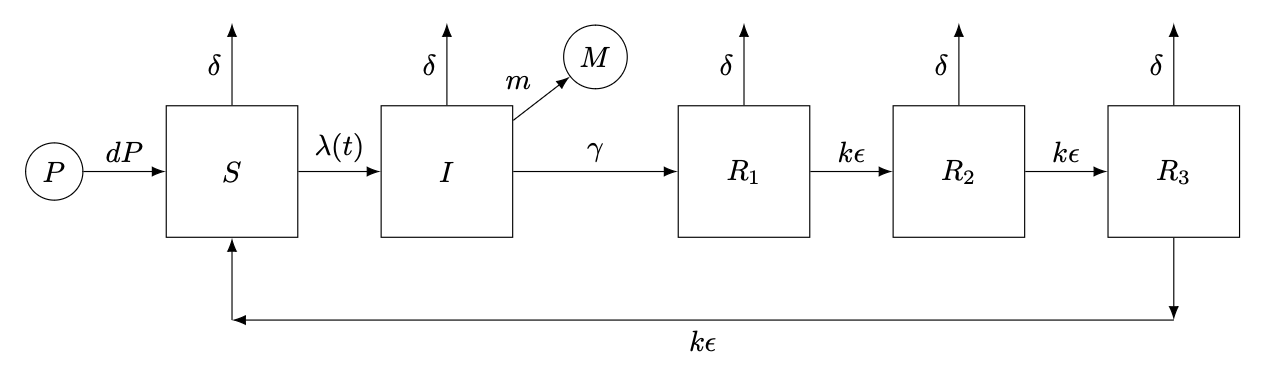
\includegraphics[width=\arxiv{14cm}{\textwidth}]{imgs/095/tikzcholera.png}
    \vspace*{-7mm}
    \caption{A compartment flow diagram for the \cite{king08} Dhaka cholera model.}
    \label{fig:tikz-cholera}
    \arxiv{}{\vspace*{-3mm}}
\end{figure}


%\subsection{Results}

We tested IFAD with $\alpha = 0$, $\alpha=0.97$ and $\alpha=1$ against IF2 on a global search problem for the Dhaka cholera model using our implementation in Pypomp 0.4.6.0 \citep{abkemeier25}.
For each method, we performed 100 searches, initialized with 100 starting parameter vectors drawn uniformly from the same wide bounding box used by \cite{ionides15}. 
To ensure a fair comparison under comparable computational effort, we ran each method for a similar amount of time.
For each method, we chose algorithmic parameters that maximized the log-likelihood well for that method while finishing within the allotted time. 
We ran IF2 for 650 iterations, while IFAD-0.97 is run using a short IF2 warm-start of 175 iterations followed by the Adam optimizer for 175 iterations.
IFAD-0 and IFAD-1 were run for 60 IF2 iterations and 225 Adam iterations.
The cooling rate used for IF2 was slower than that used for the warm start in IFAD. 
To assess whether other methods can catch up to IFAD-0.97 given more time, we separately ran the IF2-only approach for 4 times as many iterations and the IFAD variants with 4 times as many Adam iterations, slowing the cooling rate for each as well.
A summary of the optimization settings is provided in the supplement (Section~\suppSecAlgorithmicParameters), and the complete source code to reproduce the numerical results is available at \href{https://github.com/pypomp/dmop}{https://github.com/pypomp/dmop}.

\begin{table}[htbp!]
\centering
\begin{tabular}{lrrrrr}
\toprule
 & Maximum & Re-evaluated & Median & IF2 time (s) & DMOP time (s) \\
\midrule
\multicolumn{6}{l}{\textit{Comparable computational effort}} \\
\midrule
IFAD-0.97 & -3743.68 & -3744.26 & -3744.40 & 92 & 851 \\
IFAD-1 & -3744.36 & -3744.40 & -3746.84 & 35 & 902 \\
IFAD-0 & -3748.80 & -3749.02 & -3751.62 & 36 & 912 \\
IF2 & -3749.00 & -3748.97 & -3754.24 & 946 & - \\
\midrule
\multicolumn{6}{l}{\textit{Extended computational effort}} \\
\midrule
IFAD-0.97 & -3743.53 & -3744.30 & -3744.03 & 96 & 3557 \\
IFAD-1 & -3743.96 & -3744.33 & -3745.39 & 35 & 3583 \\
IF2 & -3745.97 & -3746.11 & -3752.63 & 3782 & - \\
IFAD-0 & -3748.32 & -3748.38 & -3750.37 & 35 & 3465 \\
\bottomrule
\end{tabular}

\caption{Maximum log-likelihood found by IF2 and IFAD under both comparable and extended computational effort. IFAD-0.97 performs the best among all methods.}
\arxiv{}{\vspace*{-7mm}}
\label{table:mle}
\end{table}

Our findings are summarized in Table \ref{table:mle} and Figures \ref{fig:boxplot}, \ref{fig:density}, and \ref{fig:optim}. 
Because estimating the log-likelihoods at every iteration of IF2 with particle filtering for Figure \ref{fig:optim} lengthens the computation time and thus compromises the fair comparison between methods, we obtained the times in Table \ref{table:mle} and Figure \ref{fig:optim} by running the methods again without the extra calls to the particle filter. 
Every other value displayed for the Dhaka results comes from the runs with the extra particle filter calls. 

Examining Table \ref{table:mle}, IFAD-0.97 attained a log-likelihood of -3744.17, which surpassed IF2 even when IF2 ran for 4 times as long.
IFAD-1 sometimes came close to IFAD-0.97, but its additional noise gave it worse median performance.
IFAD-1 needed to be run for an extended time for the medai log-likelihood to start catching up with IFAD-0.97.

\begin{figure}[ht]
    \centering
    \arxiv{}{\vspace*{0.1ex}}
    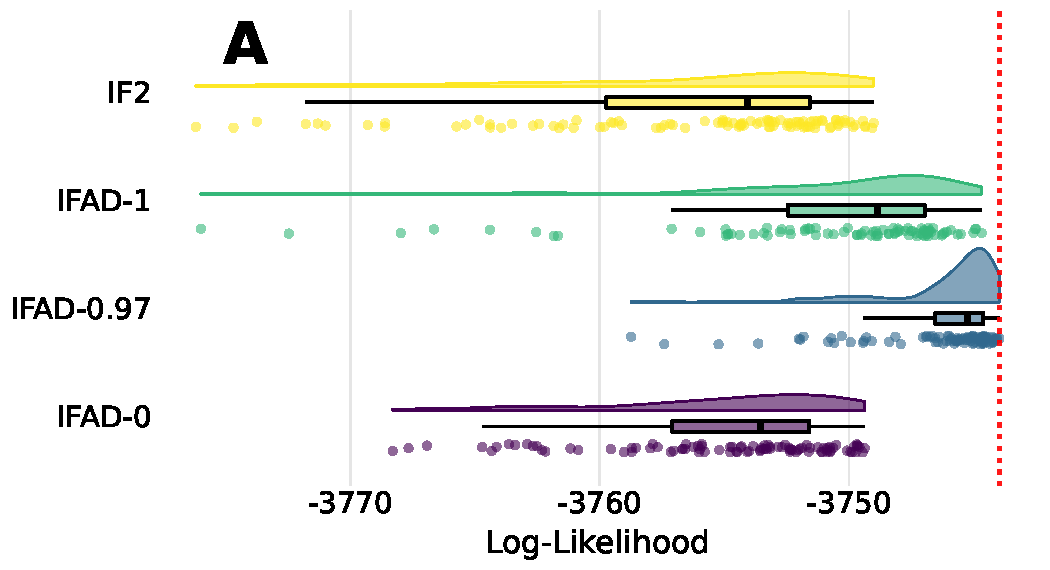
\includegraphics[width=\arxiv{0.48\textwidth}{\textwidth/\real{2.2}}]{imgs/precise_raincloud.pdf}\hfill
    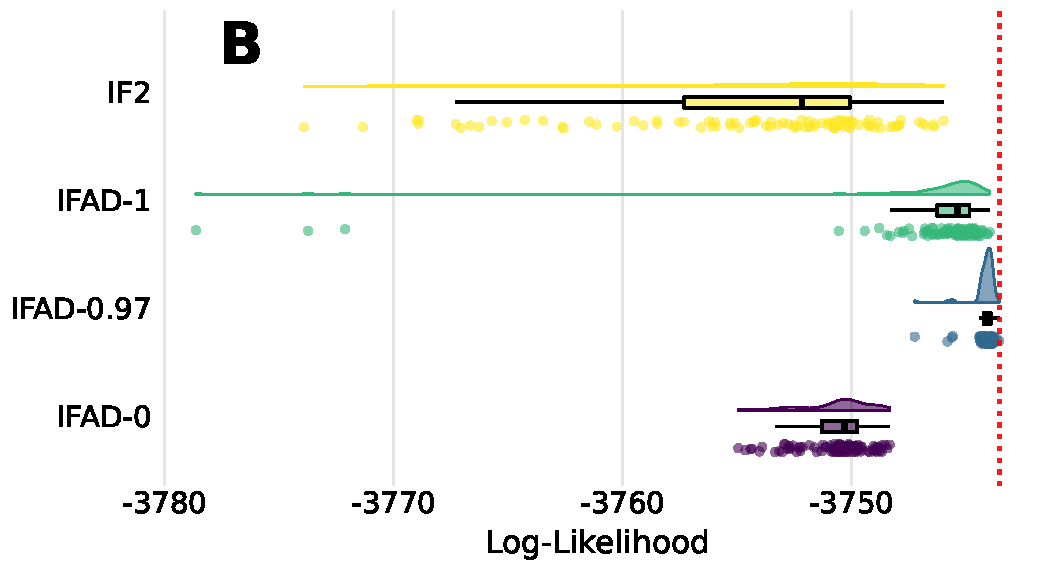
\includegraphics[width=\arxiv{0.48\textwidth}{\textwidth/\real{2.2}}]{imgs/precise_raincloud_long.pdf}
    %\arxiv{}{\vspace*{-1mm}}
    \caption{Raincloud plot of the searches. 
    \captiona\ Comparable computational effort. 
    \captionb\ Extended computational effort. 
    Log-likelihoods lower than -3800 are omitted. 
    IFAD-0.97 outperforms all other methods.
    The dotted red line shows the best-known maximized log-likelihood.}
    \label{fig:boxplot}
    \arxiv{}{\vspace*{-5mm}}
\end{figure}


\begin{figure}[htbp!]
    \centering
    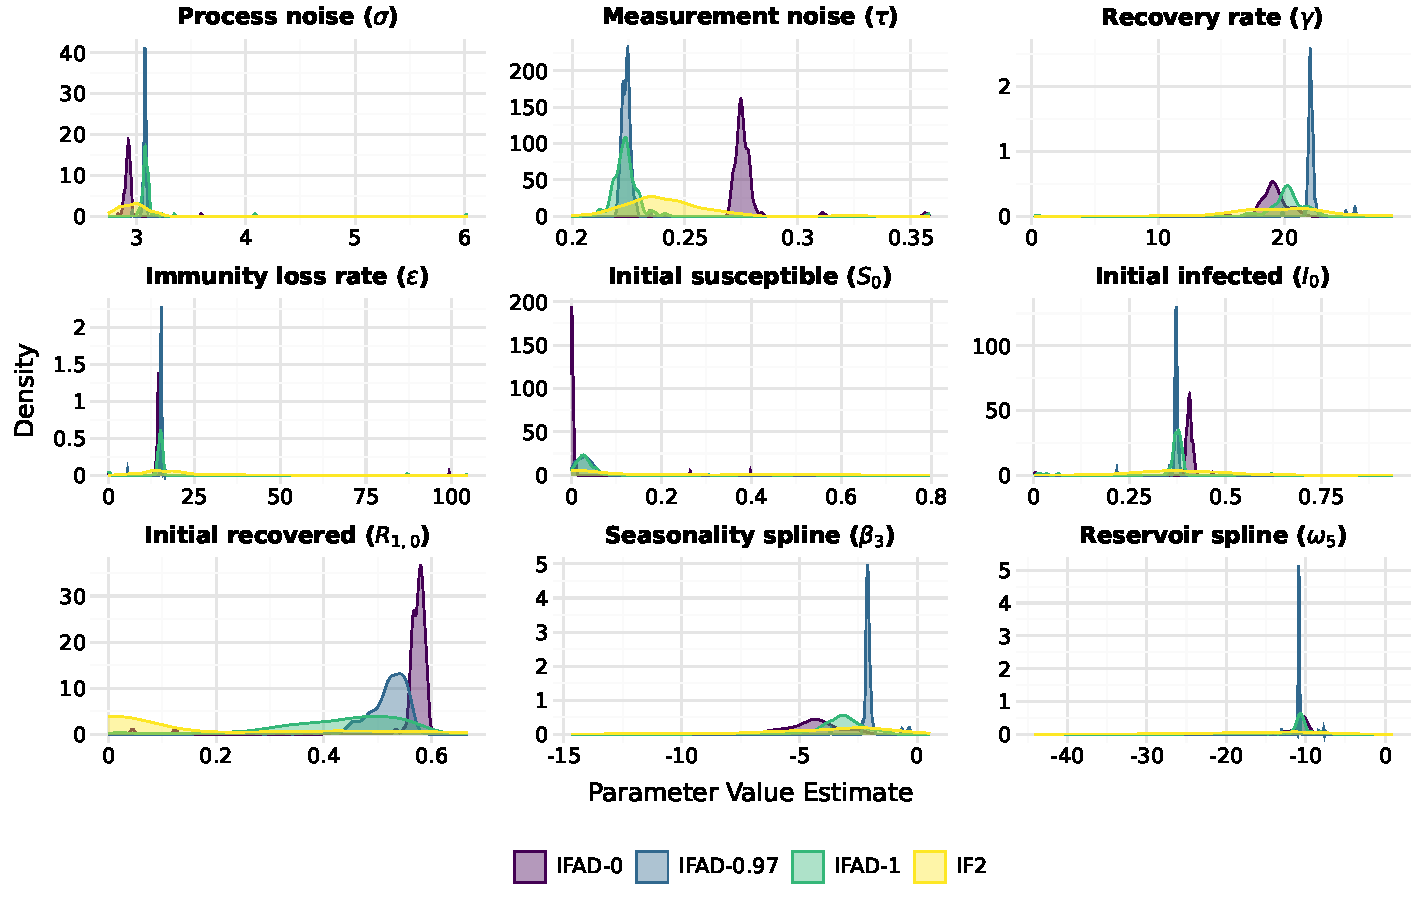
\includegraphics[width=\arxiv{14cm}{\textwidth}]{imgs/precise_density_long.pdf}
    \caption{Density plots of the final parameter estimates across the 100 replicates for nine key parameters of the cholera model under extended computational effort.}
    \label{fig:density}
\end{figure}

\begin{figure}[ht]
    \centering
    \vspace{1mm}
    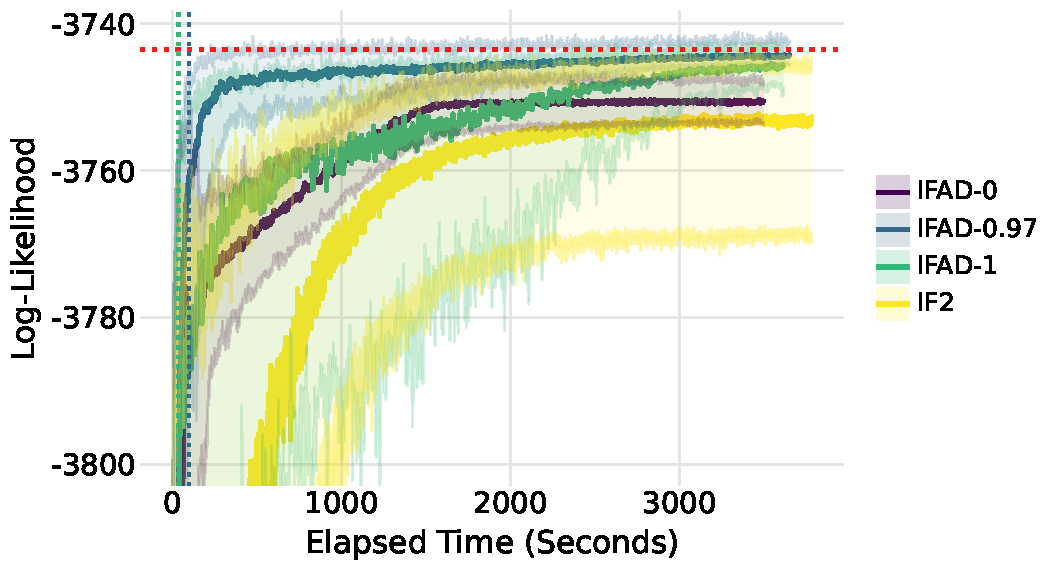
\includegraphics[width=\arxiv{14cm}{\textwidth/2}]{imgs/precise_traces_long.pdf}
    \arxiv{}{\vspace*{-1mm}}
    \caption{Optimization progress of IFAD and IF2 under extended computational effort.
    The shaded regions cover the area between the 100th and 10th percentiles of log-likelihood estimates at each iteration.
    We use a dotted red line to display the MLE.
    The vertical dotted lines indicate where the IFAD runs switch from IF2 to Adam optimization.
    Some log-likelihood estimates appear to be slightly above the MLE; this is due to Monte~Carlo evaluation error.}
    \label{fig:optim}
    \arxiv{}{\vspace*{-3ex}}
\end{figure}

 
IFAD-0 fell about 4 log-units short of IFAD-0.97 even with extended time, presumably due to its high bias. 
Based on Figure \ref{fig:optim}, IFAD-0 and IF2-only plateau heavily after being run for long enough and could not catch up to IFAD-0.97 within a reasonable timeframe.

Previously, a maximized log-likelihood of $-3748.6$ for this model and data was reported by \cite{king16}.
This MLE was obtained with much computational effort, using many global and local IF2 searches and with the assistance of likelihood profiling, 8 years after the model was first proposed by \cite{king08}.
Meanwhile, \cite{ionides15} only achieve a maximum log-likelihood of $-3768.6$, and \cite{king08} only $-3793.4$.
Using the improved computational efficiency of Pypomp (elaborated upon in Section \ref{sec:efficiency}), IF2 alone can easily surpass all of these previous results within a wall clock time of 15 minutes, and IFAD-0.97 holds the record at $-3744.17$ within a slightly shorter time. 


Notably, the log-likelihood and parameter estimates for IFAD-0.97 frequently exhibit much less Monte~Carlo variance than that of the other methods, as can be seen in Figures~\ref{fig:boxplot} and~\ref{fig:density}. 
IFAD in general exhibits less Monte~Carlo variance than IF2, especially for the parameter estimates. 
IFAD-0 has the second-lowest Monte~Carlo variance for most parameter estimates, although it has the lowest for the initial state proporitons $S_0$ and $R_{1,0}$. 
That said, the choice $\alpha=0$ is also known to have the greatest bias, and IFAD-1 agrees more closely with IFAD-0.97. 
Because multiple searches are employed to mitigate the effects of Monte~Carlo variance, the lower Monte~Carlo variance of IFAD-0.97 suggests that fewer searches are needed when running IFAD-0.97 to obtain a log-likelihood close to the maximum. 
Lowering the Monte~Carlo variance also narrows the width of Monte-Carlo-adjusted profile confidence intervals \citep{ionides17}.

%\subsection{IFAD Outperforms Both IF2 and DMOP Alone}

While IF2 effectively approaches a neighborhood of the MLE (Figure \ref{fig:optim}), IF2 alone ultimately fails to achieve the last few log-likelihood units, as IF2 struggles to get much closer than about 3 log-likelihood units of the MLE even when run for an extended time (Table \ref{table:mle}).
Conversely, we encountered many failed searches with gradient descent alone. 
This is a difficult, nonconvex, and noisy problem with $23$ estimated parameters, and gradient descent without a warm-start gets stuck in local minima and saddle points.

IFAD, by comparison, approaches the MLE quickly due to the IF2 warm-start (Figure \ref{fig:optim}) and also succeeds at refining the coarse solution found by the warm-start with DMOP gradient steps to find the MLE.
IFAD therefore successfully combines the best qualities of IF2 and DMOP, outperforming either of them alone.
Monte~Carlo replication is appropriate for IFAD, or any Monte Carlo algorithm used to solve a challenging numerical problem, but Figure~\ref{fig:optim} shows that IFAD can find higher likelihood values more quickly and more reliably than the previous state-of-the-art. 
Since replicated searches are inevitably needed for Monte~Carlo maximization of this challenging likelihood maximization task, it is important to give extra consideration to the right tail of the distributions in Figure~\ref{fig:boxplot} when comparing the capabilities of the methods. 


\section{Application to Bayesian Inference}
\label{sec:bayes}

Particle MCMC \citep{andrieu10} is arguably the most popular method for full-information plug-and-play Bayesian inference for POMP models.
However, particle Metropolis-Hastings often mixes slowly, requiring long burn-in periods.
For instance, \cite{fasiolo16} reported needing $700000$ burn-in iterations for effective sampling in the \cite{king08} model, even after coarsening each Euler timestep to reduce the computational burden. 
To alleviate this, we employ a No U-Turn Sampler (NUTS) \citep{homan14} powered by DMOP-$\alpha$, with a nonparametric empirical prior constructed from density estimation of the parameter swarm from the IF2 warm-start. 
%This prior has a standard deviation of $6.3\%$ of the MLE. 
%\sqrt{(0.02\cdot0.95^{40})^2 \cdot 600}\approx 6.3\%
Using NUTS with MOP-$\alpha$ and this prior significantly lowers the mixing time of the Markov chain to as little as $500$ iterations (Figure \ref{fig:nuts-eb}).
NUTS has been implemented with previous differentiable particle filters \citep{rosato22} but not in our plug-and-play context with control over the bias/variance tradeoff.

\begin{figure}[tb]
    \centering
    \vspace{1mm}
    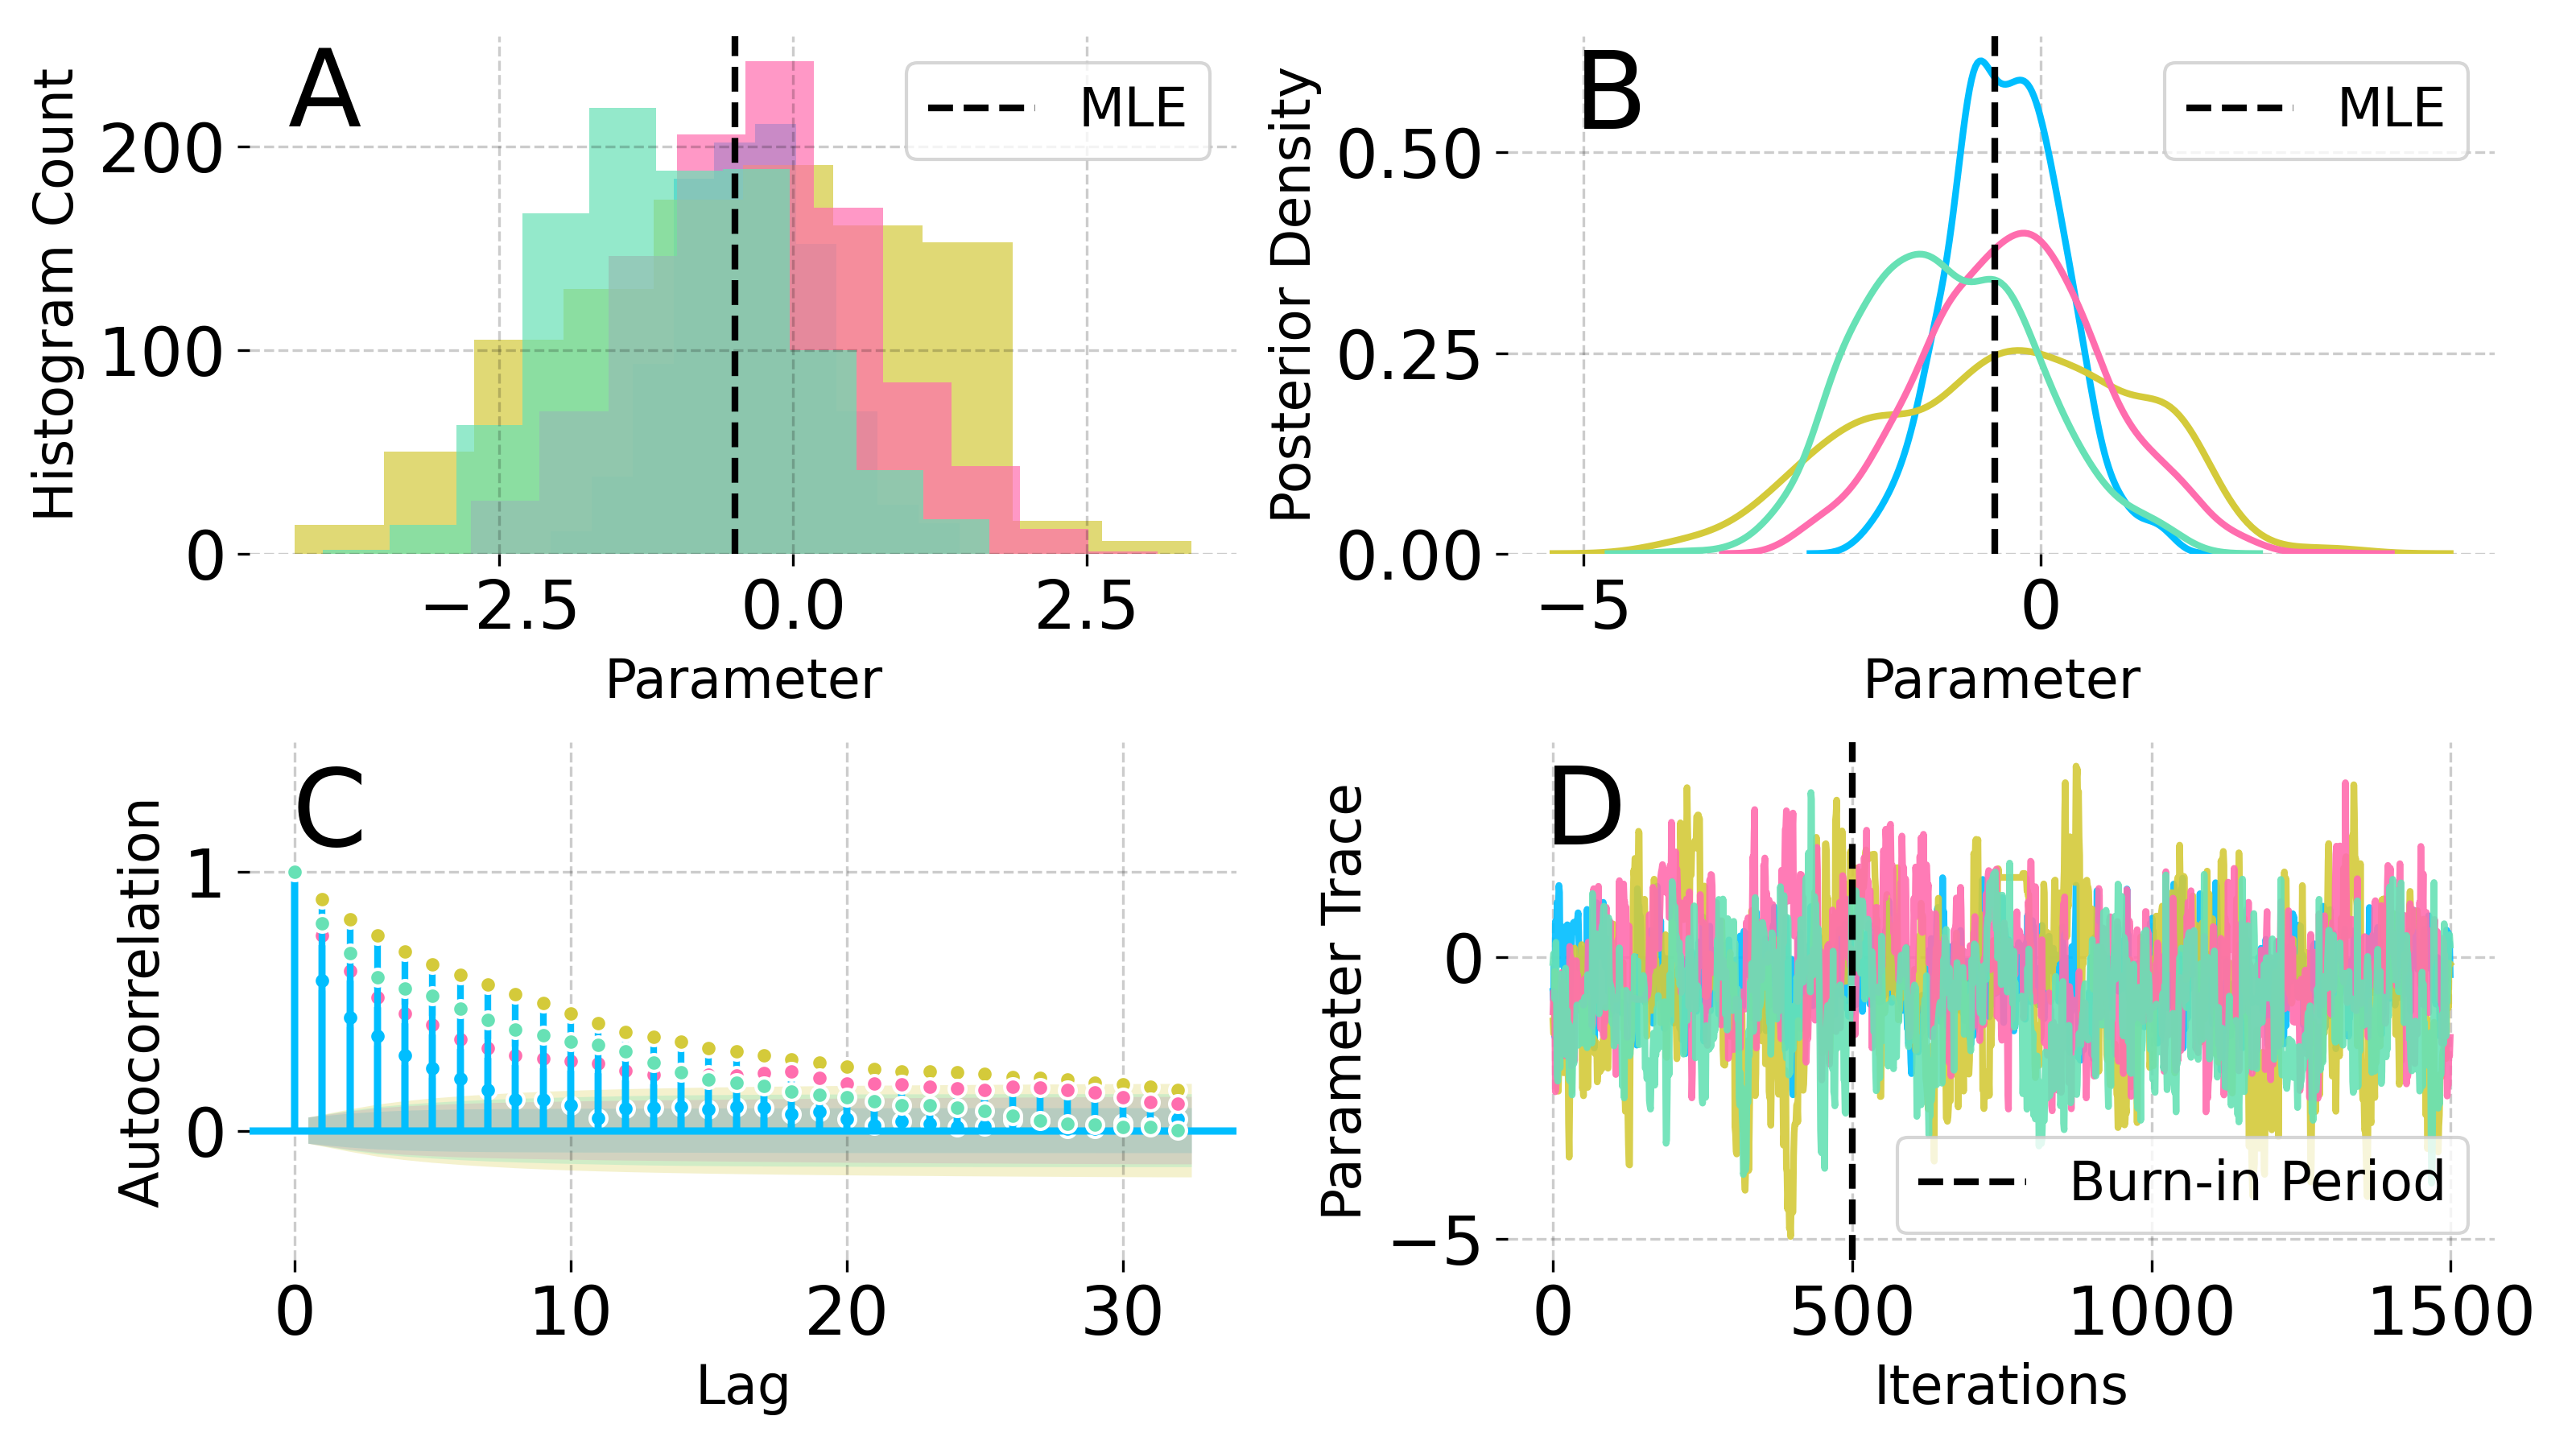
\includegraphics[width=\arxiv{\textwidth/\real{1.25}}{\textwidth}/\real{1.25}]{imgs/pmcmc/nuts_eb.png}
    \caption{Convergence diagnostics for NUTS with $4$ chains, where we plot $1000$ samples from the posterior of $\beta_{\text{trend}}$ within the Dhaka cholera model of \cite{king08}. \textbf{A:} Histogram of posterior samples. \textbf{B:} density estimate of the posterior. \textbf{C:} Autocorrelation plot for MCMC samples. \textbf{D:} Trace plot for MCMC samples, pre and post burn-in. NUTS mixes quickly when regularized by an empirical prior with a standard deviation of $6.3\%$ of the MLE, and the posterior estimates from each chain share roughly the same posterior mode.}
    \label{fig:nuts-eb}
    \arxiv{}{\vspace*{-4mm}}
\end{figure}


Without the IF2 prior, NUTS with the MOP-$\alpha$ estimate alone tended to diverge.
In contrast, particle Metropolis-Hastings, with or without said prior, fails to effectively explore the parameter space.
We display these results in the supplement (Section~\suppSecBayesFigs). 
\kevin{The sharper bias--variance analysis is Section~S7. Consequently, change the three preamble values S7, S8, and S9 for the Bayesian figures, baseline justification, and algorithmic-parameter sections to S8, S9, and S10, respectively.}
This speedup in the mixing time of particle MCMC by over three orders of magnitude provides hope that particle Bayesian inference might be increasingly employed for the complex scientific models commonly encountered in areas like epidemiology.


\section{Theoretical Analysis of MOP-$\alpha$}
\label{sec:thms}

Here, we will show that MOP-$\alpha$ targets the filtering distribution and likelihood under $\theta$, is consistent when $\alpha=1$, and characterize rates for its bias and variance under different choices of $\alpha$. To do so, we require the following assumptions:

\arxiv{}{\vspace*{-3ex}}
\begin{enumerate}[label=(A\arabic*),itemsep=-1ex, , font=\small] 
    \item \textbf{Continuity of the Likelihood.} $\ell(\theta)$ has more than two continuous derivatives in a neighborhood $\left\{\theta: \ell(\theta)>\lambda_1\right\}$ for some $\lambda_1<\sup _{\varphi} \ell(\varphi)$.\label{assump:conti-lik}
    \item \textbf{Bounded Process Model.} There exist $\underbar{M}, \bar{M}$ such that $0 < \underbar{M} \leq f_{X_n|X_{n-1}}(x_n | x_{n-1};\theta) \leq \bar{M} < \infty$.\label{assump:bounded-process}
    \item \textbf{Bounded Measurement Model.} There exist $\underbar{G}, \bar{G}$ such that $0<\underbar{G} \leq f_{Y_n \mid X_n}\left(y_n^* \mid x_n; \theta\right) \leq \bar{G}<\infty$.  In a neighborhood of the parameter under consideration, the total fixed-random-number derivatives through the reparameterized simulated state are uniformly bounded: for every $n,j$, every realization of the fixed simulator variables and reference-filter resampling indices, and all $1\leq a,b\leq p$, $|\partial_{\theta_a}^{\mathrm{tot}}\log g_{n,j}^{A,F,\theta}|\leq G'(\theta)<\infty$ and $|\partial_{\theta_a\theta_b}^{2,\mathrm{tot}}\log g_{n,j}^{A,F,\theta}|\leq G''(\theta)<\infty$.\label{assump:bounded-measurement}
    \item \textbf{Bounded Gradient Estimates.} There are functions $G(\theta), H(\theta): \Theta \to [0,\infty)$ uniformly bounded by $G^*, H^*<\infty$, such that the MOP-$\alpha$ derivatives at $\theta=\phi$ satisfy $\|\nabla_\theta\hat\ell^\alpha(\theta)\|_2\leq G(\theta)$ and $\|\nabla_\theta^2\hat\ell^\alpha(\theta)\|_{\mathrm{op}}\leq H(\theta)$ almost surely for all $\alpha$.\label{assump:local-bounded-derivative}
    \item \textbf{Differentiable Density Ratios and Simulator.} The base random-number law of the reparameterized simulator does not depend on $\theta$.  For fixed base simulator variables and fixed reference-filter resampling indices, the complete recursively simulated path and its composed log measurement densities have more than two continuous derivatives in $\theta$.\label{assump:diff-meas-and-sim}
\end{enumerate}
\arxiv{}{\vspace*{-3ex}}

\kevin{Suggested clarification to (A3) and (A5) for the Section~S7
argument.  The clarified current-function clause in (A3) should state
that, at $\theta=\phi$,
$h_n(x_n)=\nabla_\theta\log g_n^{A,F,\theta}\big|_{\theta=\phi}$
is a bounded function of the current particle location $x_n$.  The
current DMOP object is the pair consisting of $x_n$ and
$\nabla_\theta\log w_n^{F,\theta}|_{\theta=\phi}$.
Here (A2) governs the transition of $x_n$.  The algorithm first obeys
$\log w_n^{P,\theta}=\alpha\log w_{n-1}^{F,\theta}$ and then adds the
log density-ratio correction; differentiating at $\theta=\phi$ gives the
affine recursion in Section~S7 with current input $h_n(x_n)$.  Thus (A3)
bounds that current input, while
(A5) justifies its construction by fixed-random-number differentiation.
The current-function clause is the premise used by the Section~S7
coupling calculation; boundedness and differentiability alone do not
replace it.  The proof does not require total-variation mixing of the
location--log-weight-gradient pair.}

In particular, assumptions \ref{assump:bounded-process} and \ref{assump:bounded-measurement} imply that the POMP model satisfies a strong mixing condition, and as such are fairly strong but commonplace in the literature \citep{karjalainen23, delMoral04}. The fact that the likelihood estimate yielded by MOP-$\alpha$ has more than two continuous derivatives in $\theta$ follows from the construction of the likelihood estimate in equations \ref{eq:mop-conditional-likelihood} and \ref{eq:weighting-scheme}, as well as Assumptions \ref{assump:bounded-measurement} and \ref{assump:diff-meas-and-sim}. 

%\subsection{MOP-$\alpha$ Targets the Filtering Distribution}

We show that MOP-$\alpha$ targets the filtering distribution under $\theta$ and is strongly consistent for the likelihood under $\theta$ when $\alpha=1$ or $\theta=\phi$.
Employing $\alpha<1$ lead to inconsistency when $\theta$ deviates from $\phi$, but this bias disappears as $\theta$ approaches $\phi$.

While the result is presented here as specific to MOP-$\alpha$, we prove a more general result in the supplement (Section~\suppSecProofTriangularArrays).
This is a strong law of large numbers for triangular arrays of particles resampled arbitrarily, with resampling probabilities not proportional to the targeted distribution of interest, but reweighted to correct for the cumulative discrepancy between the resampling and the target distribution.


\begin{thm}[MOP-$\alpha$ Targets the Filtering Distribution and Likelihood]
    \label{thm:mop-targeting}
    When $\alpha=1$ or $\theta=\phi$, MOP-$\alpha$ targets the filtering distribution under $\theta$ and is strongly consistent for the likelihood under $\theta$. That is, for $\pi_n(\theta)=f_{X_{n}|Y_{1:n}}(x_n|y_{1:n}^* ; \theta)$ and any measurable and bounded functional $h$ and for $\hat\lik(\theta) = \prod_{n=1}^N L_n^{A,\theta,\alpha}$ or $\prod_{n=1}^N L_n^{B,\theta,\alpha}$, it holds that
    \arxiv{}{\vspace*{-1.5mm}}
    \begin{equation} \nonumber
        \frac{\sum_{j=1}^J h(x_{n,j}^{F, \theta}) \, w_{n,j}^{F,\theta}}{\sum_{j=1}^J w_{n,j}^{F,\theta}} \stackrel{a.s.}{\to} E_{\pi_n(\theta)} \big[h(X_n)\big], \hspace{5mm} \hat\lik(\theta)  \stackrel{a.s.}{\to} \lik(\theta).
    \arxiv{}{\vspace*{-1.5mm}}
    \end{equation}
\end{thm}

\begin{proof}[Proof.]
    We provide a proof sketch here, deferring the details to the supplement (Section~\suppSecProofTriangularArrays). 
    When $\theta=\phi$, the ratio ${g_{n,j}^\theta}/{g_{n,j}^\phi}=1$ regardless of $\alpha$, reducing to the vanilla particle filter.
    When $\alpha=1$ and $\theta\neq\phi,$ suppose inductively that $\{(X^{F,\theta}_{n-1,j},w^{F,\theta}_{n-1,j})\}_{j=1}^J$ targets $f_{X_{n-1}|Y_{1:n-1}}(x_{n-1}|y^*_{1:n-1};\theta)$.
    It can then be shown that $\{(X^{P,\theta}_{n,j},w^{P,\theta}_{n,j})\}_{j=1}^J$ targets $f_{X_{n}|Y_{1:n-1}}(x_{n}|y^*_{1:n-1};\theta)$, that $\{(X^{P,\theta}_{n,j},w^{P,\theta}_{n,j} \, g^\theta_{n,j} )\}_{j=1}^J$ targets  $f_{X_{n}|Y_{1:n}}(x_{n}|y^*_{1:n};\theta)$, and that weighting the particles by $(X^{F,\theta}_{n,j},w^{F,\theta}_{n,j}) = (X^{P,\theta}_{n,k_j}, w^{P,\theta}_{n,k_j} \, g^\theta_{n,k_j} \big/ g^\phi_{n,k_j})$,
    resampling the $k_j$ with probabilities proportional to $g^\phi_{n,j}$, also targets $f_{X_{n}|Y_{1:n}}(x_{n}|y^*_{1:n};\theta)$.
    Estimating the likelihood with the before-resampling estimator $\hat\lik(\theta) = \prod_{n=1}^N L_n^{B,\theta,\alpha}$, we see that the strong consistency is a direct consequence of our result that $\{ \big(X^{P,\theta}_{n,j},w^{P,\theta}_{n,j}\big) \}$ targets $f_{X_{n}|Y_{1:n-1}}(x_{n}|y^*_{1:n-1};\theta)$. 
\end{proof}


%\subsection{DMOP-$1$ Score Estimate Is Consistent}

We take advantage of the equivalence between DMOP-$\alpha$ and the derivative of MOP-$\alpha$ to investigate the former by studying the latter.
Although we have shown the DMOP-$1$ gradient estimate yields the estimate of \cite{poyiadjis11} and \cite{scibior21} when applied to the bootstrap filter, those authors estimate the Fisher score by 
$\frac{1}{J}\sum_{j=1}^J \nabla_\theta \log f_{X_{0:N}, Y_{1:N}}(x_{0:n,j}^{A, F,\theta}, y_{1:N}^* ; \theta)$ and not
$\frac{1}{J}\sum_{j=1}^J \nabla_\theta \log f_{Y_{1:N}| X_{1:N}}(y_{1:N}^* | x_{1:n,j}^{A, F,\theta}; \theta).$
It is therefore not immediately apparent that these two converge to the same thing.
As such we directly show the consistency of the MOP-$1$ gradient estimate below. 

\begin{thm}[Consistency of MOP-$1$ Gradient Estimate]
    The gradient estimate of MOP-$\alpha$ when $\alpha=1$, $\theta=\phi$ is strongly consistent for the score: $\nabla_\theta \hat\ell_J^1(\theta) \stackrel{a.s.}{\to} \nabla_\theta \ell(\theta)$ as $J \to \infty$.
    \label{thm:mop-grad-consistency}
\end{thm}

We present a proof outline here, postponing the full argument to the supplement (Section~\suppSecProofConsistency).
Assumption \ref{assump:local-bounded-derivative} lets us show uniform equicontinuity of the sequence for almost every $\omega \in \Omega$, allowing us to apply Arzela-Ascoli and Theorem \ref{thm:mop-targeting} to establish uniform convergence for the derivatives as a sequence $(\nabla_\theta \hat\lik_J^1(\theta)(\omega))_{J \in \mathbb{N}}$. This is a sufficient condition for swapping the limit and derivative to show that for almost every $\omega \in \Omega$, $\lim_{J \to \infty} \nabla_\theta \hat\lik_J^1(\theta)(\omega) = \nabla_\theta \lim_{J \to \infty} \hat\lik_J^1(\theta)(\omega) = \nabla_\theta \lik(\theta).$


%\subsection{DMOP-$\alpha$ Error, Bias and Variance}

We now provide a result showing that DMOP-$\alpha$ has a desirable bias-variance tradeoff when $0<\alpha<1$.
This is achieved because it combines favorable properties from the low-variance but asymptotically biased estimate of \cite{naesseth18} and the high-variance but consistent estimate of \cite{poyiadjis11}. 
As the bias itself is difficult to analyze, we instead analyze the MSE and variance. 
The below result applies for any $\alpha \in [0,1)$, but not $\alpha=1$, as the gradient estimate when $\alpha=1$ has no forgetting properties. 

\begin{thm}[MSE and Variance of DMOP-$\alpha$]
    \label{thm:mop-biasvar}
    When $\alpha\in (0,1)$ and $\theta=\phi$, define $\psi_k(\alpha)=(\alpha^k  + \alpha^{k+1} - \alpha)/(1-\alpha)$. 
    There exists an $\epsilon>0$ depending on $\bar{M}, \underbar{M}, \bar{G}, \underbar{G}$ as in \cite{karjalainen23} such that the MSE and variance of DMOP-$\alpha$ are:
    \vspace*{-1ex}
    \arxiv{\begin{eqnarray}
        \E\big\|\nabla_\theta\ell(\theta) - \nabla_\theta \hat\ell^\alpha(\theta)\big\|_2^2 
        &\lesssim& \min_{k \leq N} Np \, G'(\theta)^2\left(k^2J^{-1}+(1-\epsilon)^{\floor{k/(c\log(J))}}+k+\psi_k(\alpha)\right), \label{eq:mop-mse}
        \\
        \Var\big(\nabla_\theta \hat\ell^{\alpha}(\theta)\big) &\lesssim& \min_{k\leq N} Np \, G'(\theta)^2\left(\frac{k^2}{(1-\alpha)^2J} + \frac{\alpha^{k}}{1-\alpha}N\right). \label{eq:mop-variance}
        \end{eqnarray}}{\begin{align}
        &\E\big\|\nabla_\theta\ell(\theta) - \nabla_\theta \hat\ell^\alpha(\theta)\big\|_2^2 \label{eq:mop-mse}\\
        &\lesssim \min_{k \leq N} Np \, G'(\theta)^2\left(k^2J^{-1}+(1-\epsilon)^{\floor{k/(c\log(J))}}+k+\psi_k(\alpha)\right), \nonumber 
        \\
        &\Var\big(\nabla_\theta \hat\ell^{\alpha}(\theta)\big) \lesssim \min_{k\leq N} Np  G'(\theta)^2\left(\frac{k^2}{(1-\alpha)^2J} + \frac{\alpha^{k}}{1-\alpha}\right). \label{eq:mop-variance}
        \end{align}}
\end{thm}
\arxiv{}{\vspace*{-1ex}}

\kevin{Suggested replacement for Theorem~\ref{thm:mop-biasvar}.
Under (A2), the clarified forms of (A3) and (A5), fixed observations,
multinomial resampling, $J\geq2$, $\theta=\phi$, and $\alpha\in[0,1)$,
the following bounds hold.  Here the current DMOP object consists of the
particle location and the gradient of its log weight.  The location transition
is the one in (A2), the current measurement-gradient input is the bounded
function in (A3), and differentiating the log-space weight recursion gives
$\nabla_\theta\log w_n^{F,\theta}
=\alpha\nabla_\theta\log w_{n-1}^{F,\theta}+h_n(x_n)$ at
$\theta=\phi$ along a selected lineage.  No total-variation minorization of
this pair is assumed.  Then
\[
\E\|\nabla_\theta\hat\ell^\alpha(\theta)
-\nabla_\theta\ell^\alpha(\theta)\|_2^2,
\quad
\Var\{\nabla_\theta\hat\ell^\alpha(\theta)\}
\lesssim
pG'(\theta)^2\left\{
\frac{N}{J(1-\alpha)^2}
+\frac{N^2}{J^2(1-\alpha)^2}
\right\}.
\]
Consequently,
\[
\E\|\nabla_\theta\hat\ell^\alpha(\theta)
-\nabla_\theta\ell(\theta)\|_2^2
\lesssim pG'(\theta)^2\left[
\frac{N}{J(1-\alpha)^2}
+\frac{N^2}{J^2(1-\alpha)^2}
+\left\{
\sum_{r=1}^{N-1}(N-r)(1-\alpha^r)\varrho^r
\right\}^2\right].
\]
Here $\varrho\in(0,1)$ is independent of $N,J$, and $\alpha$.  The exact
bias--variance identity also holds, and the population discount bias is
bounded by
\[
\|\nabla_\theta\ell^\alpha(\theta)-\nabla_\theta\ell(\theta)\|_2
\leq
C\sqrt p\,G'(\theta)
\sum_{r=1}^{N-1}(N-r)(1-\alpha^r)\varrho^r
\leq
CN\sqrt p\,G'(\theta)
\frac{\varrho(1-\alpha)}
{(1-\varrho)(1-\alpha\varrho)}.
\]
The $N^2/J^2$ term is the quadratic self-normalized-ratio remainder, not
an additional oscillation normalization of the full score.  If $J\geq N$,
it is absorbed by the $N/J$ term in the coarser display.  Lemma~S13 proves
the sharper lag-moment bound
\[
\E\|\nabla_\theta\hat\ell^\alpha-\nabla_\theta\ell^\alpha\|_2^2,
\quad
\Var(\nabla_\theta\hat\ell^\alpha)
\lesssim
pG'(\theta)^2
\left(\frac NJ+\frac{N^2}{J^2}\right)
\frac{1+\alpha\varrho}
{(1-\alpha^2)(1-\alpha\varrho)}.
\]
At $\alpha=1$, the corresponding finite-horizon bound is
$pG'(\theta)^2\min\{N^2,N^2/J+N^3/J^2\}$.  The proof conditions on the particle
locations but not on the realized ancestral indices and uses the exact
backward genealogy representation of \citet{chanDelMoral18}; (A2) then
minorizes every backward kernel and gives geometric lag covariance.}

\kevin{Interpretation of the third MSE term.  Its sharper finite-horizon
upper-bound contribution is
\[
pG'(\theta)^2
\left\{\sum_{r=1}^{N-1}(N-r)(1-\alpha^r)\varrho^r\right\}^2.
\]
The factor $\varrho^r$ is therefore present.  The remaining
$1-\alpha$ order cannot be improved uniformly under the stated
assumptions, although particular models can have signed first-order
cancellation.  The identity follows because $\alpha^r$ is the survival
probability of a geometric cutoff
with probabilities $(1-\alpha)\alpha^k$, including probability
$1-\alpha$ of cutoff zero.  Algebraically,
\[
\sum_{r\geq1}(1-\alpha^r)\varrho^r
=\sum_{k\geq0}(1-\alpha)\alpha^k
  \frac{\varrho^{k+1}}{1-\varrho}
=\frac{\varrho(1-\alpha)}
{(1-\varrho)(1-\alpha\varrho)}.
\]
Thus one cannot replace this expression by
$C\varrho^{\alpha/(1-\alpha)}$ uniformly as $\alpha\uparrow1$ with
$C$ independent of $\alpha$.  Since
$\alpha/(1-\alpha)=1/(1-\alpha)-1$, using $1/(1-\alpha)$ as the
effective horizon changes the proposed exponential rate only by a fixed
factor.  More strongly, for fixed $N$, the exact fixed-data discrepancy is
a finite polynomial in $1-\alpha$.  For some $c>0$, an upper bound of order
$\varrho^{c/(1-\alpha)}$ would force every coefficient of that polynomial
to vanish, so the discrepancy would be identically zero.
The comparison is nevertheless favorable when $\alpha$ is calibrated to
the mixing time.  Put $k=\lfloor\alpha/(1-\alpha)\rfloor$, the integer
part of the mean geometric time.  The ratio of the geometric scalar bound
to the fixed-lag scalar bound is
\[
\frac12<
\frac{(1-\alpha)\varrho^{-k}}{1-\alpha\varrho}
\leq\varrho^{-k},
\]
provided $k<N$ so that the horizon has not saturated.  The lower bound
follows by retaining the first $k+1$ terms in the geometric-series
representation, which gives $1-\alpha^{k+1}>1/2$.  Thus the two uncapped
bounds differ by at most a fixed factor when
$k|\log\varrho|$ is bounded, meaning that discount memory spans at most a
fixed number of mixing e-folding times.  This provides a finite-regime
explanation consistent with comparable empirical behavior; the asymptotic
gap appears when $\alpha\uparrow1$ with $\varrho$ fixed.
There is also a sharper result when expectation is taken over observations
generated from the original POMP at $\theta_0$, so that
$Y_n\mid X_n\sim f_{Y_n\mid X_n}(\mathord\cdot\mid X_n;\theta_0)$,
rather than conditioning on the realized values $y_{1:N}^*$.  This
introduces no second observation model.  The per-time difference between
the exact and DMOP-$\alpha$ population scores then has conditional mean zero
given the previous observations.  Its cross-time inner products therefore
vanish, and the final remark of Section~S7 states explicitly that
\[
\E_{\theta_0}\|\nabla_\theta\ell^\alpha(\theta_0)
-\nabla_\theta\ell(\theta_0)\|_2^2
\leq
CNpG'(\theta_0)^2
\left\{\frac{\varrho(1-\alpha)}
{(1-\varrho)(1-\alpha\varrho)}\right\}^2,
\]
provided the lagwise bound is uniform over the random observations, or has
a random per-time bound whose second moment is uniformly bounded in $n$.
Hence the third term accumulates as $N$, not $N^2$, for data-averaged score
MSE.  Moreover, for every fixed
$\alpha$, the population score remains an unbiased estimating equation;
the parameter estimator retains the usual $N^{-1/2}$ rate, with a possible
sandwich-efficiency loss rather than a loss of consistency rate.  The same
remark also displays the mixing-calibrated comparison for
$k=\lfloor\alpha/(1-\alpha)\rfloor$.}

We provide an outline, deferring the full proof to the supplement (Section~\suppSecProofBiasVar).
The variance bound can be reduced to the approximation error between the score estimate from DMOP-$\alpha$ and a variant called DMOP-$(\alpha,k)$ where the discounted weights are truncated at lag $k$. 
The discount factor, $\alpha$, ensures strong mixing.
The covariance of the derivative of MOP-$(\alpha,k)$ are controlled with Davydov's inequality and a standard $L^p$ error bound for the particle filter. 
The MSE bound considers the error between the target derivative and DMOP-$(1,k)$, and the error between DMOP-$(1,k)$ and DMOP-$\alpha$. 
The latter can be shown to be $\tilde{O}\big(Np \, G'(\theta)^2(k+\psi_k(\alpha))\big)$, and the former can be controlled with a result on the the forgetting of the particle filter from \cite{karjalainen23} and the very same $L^p$ error bound mentioned above. 

\kevin{Suggested replacement proof outline.
The clarified (A3) and (A5) justify differentiation under each finite-horizon
simulator expectation.
Posterior backward-kernel contraction gives geometric decay of the population lag
coefficients and hence the population discount bias.
A local Del Moral--Rio perturbation expansion is then applied to each
continuation ratio before summing over discounted observation times.  Conditional
multinomial centering makes the first-order local fields martingale differences,
The exact conditional backward representation of a sampled particle genealogy
from \citet{chanDelMoral18}, together with (A2), gives
\[
|\Cov\{h_s(X_s),h_u(X_u)\mid\hbox{particle locations}\}|
\lesssim G'(\theta)^2\varrho^{|s-u|}.
\]
Consequently, the centered squared contributions sum to order
$N/\{J(1-\alpha^2)\}$ before horizon saturation.  The same backward
martingale calculation gives the fourth moment needed for the quadratic
ratio remainders, improving their contribution to
$N^2/\{J^2(1-\alpha^2)\}$.  The current object used in
this calculation consists of the location and the gradient of its log weight.
Assumption (A2) couples the location component geometrically, while
differentiation of the log-space weight recursion multiplies the inherited
gradient by $\alpha$ and adds $h_n(x_n)$.  Full-score
summation by parts gives
\[
(1-\alpha)\sum_{r=q}^{L-1}\alpha^{r-q}+\alpha^{L-q}=1,
\]
so a previously accumulated difference contracts by $\alpha$, every new
$h_n(x_n)$ difference is summable under location coupling, and no additional
mixing-time factor appears.  More directly, if two locations are coupled
so that their probability of disagreement after $r$ steps is at most
$\varrho^r$, then
\[
\E|w_{t+r}-w'_{t+r}|
\leq\alpha^r|w_t-w'_t|
+2G'(\theta)\sum_{q=1}^r\alpha^{r-q}\varrho^q,
\]
which decays at rate $\max(\alpha,\varrho)^r$, apart from the factor $r$
when $\alpha=\varrho$.  The proof therefore needs no total-variation
contraction assumption for the pair.  The uniform $J^{-1}$ current-filter
weak-bias lemma is not applied directly to a historical genealogical
functional.}
\kevin{Audit of the other SI variance arguments.
The DMOP-$0$ calculation remains valid because no historical score is carried
across resampling times.  The earlier fixed-lag calculation does not remain valid:
in the exact constant-weight model its variance has order $N(k+1)/J$ for
$1\ll k\ll\min(N,J)$ and order $N^2/J$ at $k=N-1$, rather than
$\{N+(k+1)^2\}/J$.  The current DMOP pair includes the particle location and
the gradient of its log weight.  The backward genealogy calculation in
Lemma~S13 now controls covariance among score contributions that share a
resampling genealogy and recovers the $N(k+1)/J$ leading upper bound, with
the corresponding second-order particle term.  It does not identify an
ancestral sum with a current-location function.}


Theorem \ref{thm:mop-biasvar} provides theoretical understanding of the empirically favorable bias-variance tradeoff enjoyed by DMOP-$\alpha$ in Figure \ref{fig:biasvar}.
The first term in the MSE bound in Equation \ref{eq:mop-mse} corresponds to particle approximation error, the second mixing error, and the third and fourth the error between the DMOP-$(1,k)$ and DMOP-$\alpha$ score estimates. 
As $\alpha$ goes to $1$, choosing $k$ appropriately, the first, third and fourth term (corresponding to the variance) increases, while the second term (corresponding to the bias) decreases. 
Likewise, the first term in the variance bound in Equation \ref{eq:mop-variance} corresponds to particle approximation error, while the second corresponds to mixing error. 
The variance increases as $\alpha$ goes to $1$. 


%\subsection{Bias-Variance Tradeoff}

We show in Section~{\suppSecProofBiasVar} that the variance of DMOP-$0$ is $\tilde{O}\big( Np \, G'(\theta)^2\big/J \big)$.
Previously, \cite{poyiadjis11} established that the variance of DMOP-$1$ is $\tilde{O}(N^4/J)$, ignoring factors of $p$ and $G'$. 
Combining these results with Theorem \ref{thm:mop-biasvar} shows that DMOP-$\alpha$ interpolates between the variances of DMOP-$0$ and DMOP-$1$, as $N \leq Nk^2 \leq N^4$, with a phase transition as soon as $\alpha<1$. 
The phase transition arises because even though the particle filter has forgetting properties \citep{karjalainen23}, the resulting derivative estimate of \cite{poyiadjis11} does not, and we require both for the variance reduction. 

DMOP-$\alpha$ achieves a lower MSE than DMOP-$1$, as $\alpha, k$ can be as large as desired to balance the impact of the last three terms of Equation \ref{eq:mop-mse}.
We also show that DMOP-$0$ achieves a MSE of $\tilde{O}\big(NpG'(\theta)^2(J^{-1}+(1-\epsilon)^{\lfloor1/c\log(J)\rfloor})\big)$, where the second term corresponds to uncontrolled mixing error.
Unlike DMOP-$\alpha$, DMOP-$0$ has no opportunity to tune $\alpha$ (or $k$) to reduce said mixing error, leading to uncontrolled asymptotic bias. 

\kevin{Suggested correction to this endpoint discussion.
Theorem~1 of \citet{poyiadjis11} gives a quadratic lower bound for the
central-limit asymptotic variance of their already unnormalized additive path
estimator; no additional $N^2$ normalization factor should be applied.
A separate generic norm-one path-space RMSE bound of order $N/\sqrt J$ becomes
$N^2/\sqrt J$, and hence $N^4/J$ in MSE, after rescaling by the
$O(N)$ oscillation of the full unnormalized score.
That quartic quantity is a generic upper bound, not the Poyiadjis lower-bound rate.
DMOP-$1$'s reparameterization score contributions are not generally particlewise
identical to the complete-data likelihood-ratio score contributions of
\citet{poyiadjis11}, so their lower bound
does not automatically transfer to DMOP-$1$.
There is also no DMOP-$0$ MSE lower bound under the present assumptions.
For $\alpha<1$, Lemma~S13 gives the sharper particle term proportional to
$(1-\alpha^2)^{-1}$.  Balancing it against the fixed-observation population
term gives
\[
1-\alpha\asymp
\left(\frac1{NJ}+\frac1{J^2}\right)^{1/3}.
\]
Before horizon saturation, the resulting MSE upper bounds are
$pG'(\theta)^2N^2/J^{4/3}$ when $J\lesssim N$ and
$pG'(\theta)^2N^{4/3}/J^{2/3}$ when
$N\lesssim J\lesssim N^2$.  Once $J\gtrsim N^2$, a choice
$1-\alpha\asymp J^{-1/2}$ gives the finite-horizon upper bound
$pG'(\theta)^2N^2/J$.  These are only bounds obtained by balancing the
proved upper bound.  The signed population
bias can cancel, so neither this calculation nor the endpoint bounds prove that
the actual MSE has, or lacks, an interior minimizer.}



\section{Computational Efficiency} \label{sec:efficiency}

DMOP-$\alpha$ and IFAD are fast algorithms, both in theory and practice: the cheap gradient principle of \cite{kakade2019provably} suggests that a gradient estimate from DMOP-$\alpha$ should take no more than 6 times that of the runtime of the particle filter.
We found the empirical value of this factor to be 3.75, using the implementation of our methods in the Pypomp library \citep{abkemeier25}.
DMOP-$\alpha$ and IFAD therefore share the same $O(NJ)$ time complexity as the particle filter, unlike the $O(NJ^2)$ complexity of \cite{corenflos21} and Algorithm 2 in \citep{poyiadjis11, scibior21}.

Implementation of the particle filter, IF2, and DMOP-$\alpha$ in JAX \citep{jax} takes advantage of just-in-time compilation and GPU acceleration.
While CPU-based implementations of the particle filtering methods can effectively leverage multiple cores by parallelizing over independent replications of a given method, Pypomp can effectively leverage tens of thousands of GPU cores by vectorizing over both particles and independent method replications.
To examine the performance improvement on the Dhaka model, we ran 1 instance of IF2 with 60 iterations and 5000 particles using 1 CPU core and compared this with running 100 replications on a GPU.
The results in Table \ref{table:speedup} show that, despite running 100 times as many replications, the GPU finishes 10.4 times faster, giving it a throughput 1038.9 times greater than the single CPU core.

\begin{table}[htbp!]
\centering
\begin{tabular}{lll}
\toprule
Metric & \texttt{pomp} \citep{king16} & Pypomp \citep{abkemeier25} \\
\midrule
Language & R (C simulator) & Python (JAX) \\
Hardware& 3.0 GHz Intel Xeon Gold 6154 (1 core) & NVIDIA RTX6000 Pro Blackwell \\
IF2 Replications & 1 & 100 \\
Latency (s) & 935 & 90 \\
\bottomrule
\end{tabular}
\caption{Comparison of execution latency for running IF2 (60 iterations, 5000 particles, 1 versus 100 replications) between the \texttt{pomp} (CPU-only, R and compiled C) and Pypomp (GPU-accelerated, compiled Python).}
\label{table:speedup}
\end{table}




\section{Discussion}

Practical likelihood-based data analysis involves many likelihood optimizations \citep{king08,blake14,pons-salort18,subramanian21,fox22,drake23}.
This occurs with profile likelihood confidence intervals and model selection. A careful scientist should consider many model variations, to see whether the conclusions of the study are sensitive to alternative model specifications.
Coding model variations is relatively simple when using plug-and-play inference methodology.
However, assessing the scientific potential of these variations requires likelihood optimization.
Monte~Carlo adjusted profile methods can help to acommodate maximization and evaluation error \citep{ionides17,ning21} but these methods are most effective when the maximized log-likelihood can be obtained within a few units.
Improving the process of model fitting has practical consequences for the ability of scientists to evaluate hypotheses.
We have demonstrated, for the first time, a plug-and-play maximum likelihood approach which provides a high-quality log-likelihood maximization in the complex benchmark model of \cite{king08}.
We anticipate that this will promote scientific advances in all domains where complex POMP models arise.


If the simulator is discontinuous in $\theta$, DMOP-$\alpha$ no longer applies.
We are working on a variation of DMOP-$\alpha$ applicable to this case.
Specifically, differentiable transition density ratios can be used instead of a differentiable simulator.
The off-parameter treatment of the measurement model is extended to an off-parameter simulation for the dynamic process.
In that case, one requires access to the transition densities, or at least their ratios. 
This algorithm may be better suited to large discrete state spaces than either DMOP-$\alpha$ or differentiation of the Baum-Welch algorithm.

Discounting the weights by some $\alpha \in [0,1]$ is not the only way to interpolate between the estimators of \cite{naesseth18} and \cite{poyiadjis11}. 
As the proof of Theorem \ref{thm:mop-biasvar} implies, we can also truncate the weights at a fixed lag, corresponding to the MOP-$(1,k)$ algorithm mentioned. 
The analysis is similar, with comparable rates but with a slightly less convenient implementation. 


\section*{Acknowledgments}
This research was supported by National Science Foundation grants DMS-1761603 and DEB-1933497. 
We thank Nicolas Chopin for communications regarding the strong law of large numbers for off-parameter resampled particle filters, and other feedback. We thank Jun Chen, Arnaud Doucet and Kunyang He for helpful discussions regarding the manuscript.


%\bibliographystyle{abbrvnat}
\bibliographystyle{apalike}
% Bibliography
\bibliography{bib-ifad}

\end{document}
